\chapter{Tests Performed, Results and Discussion} \label{chap:tests}
\section{Phase I: Determining Moduli of Elasticity}
\subsection{Bending Tests}
\begin{figure} [H]
\centering
	\caption{Test Fixture and Software}
	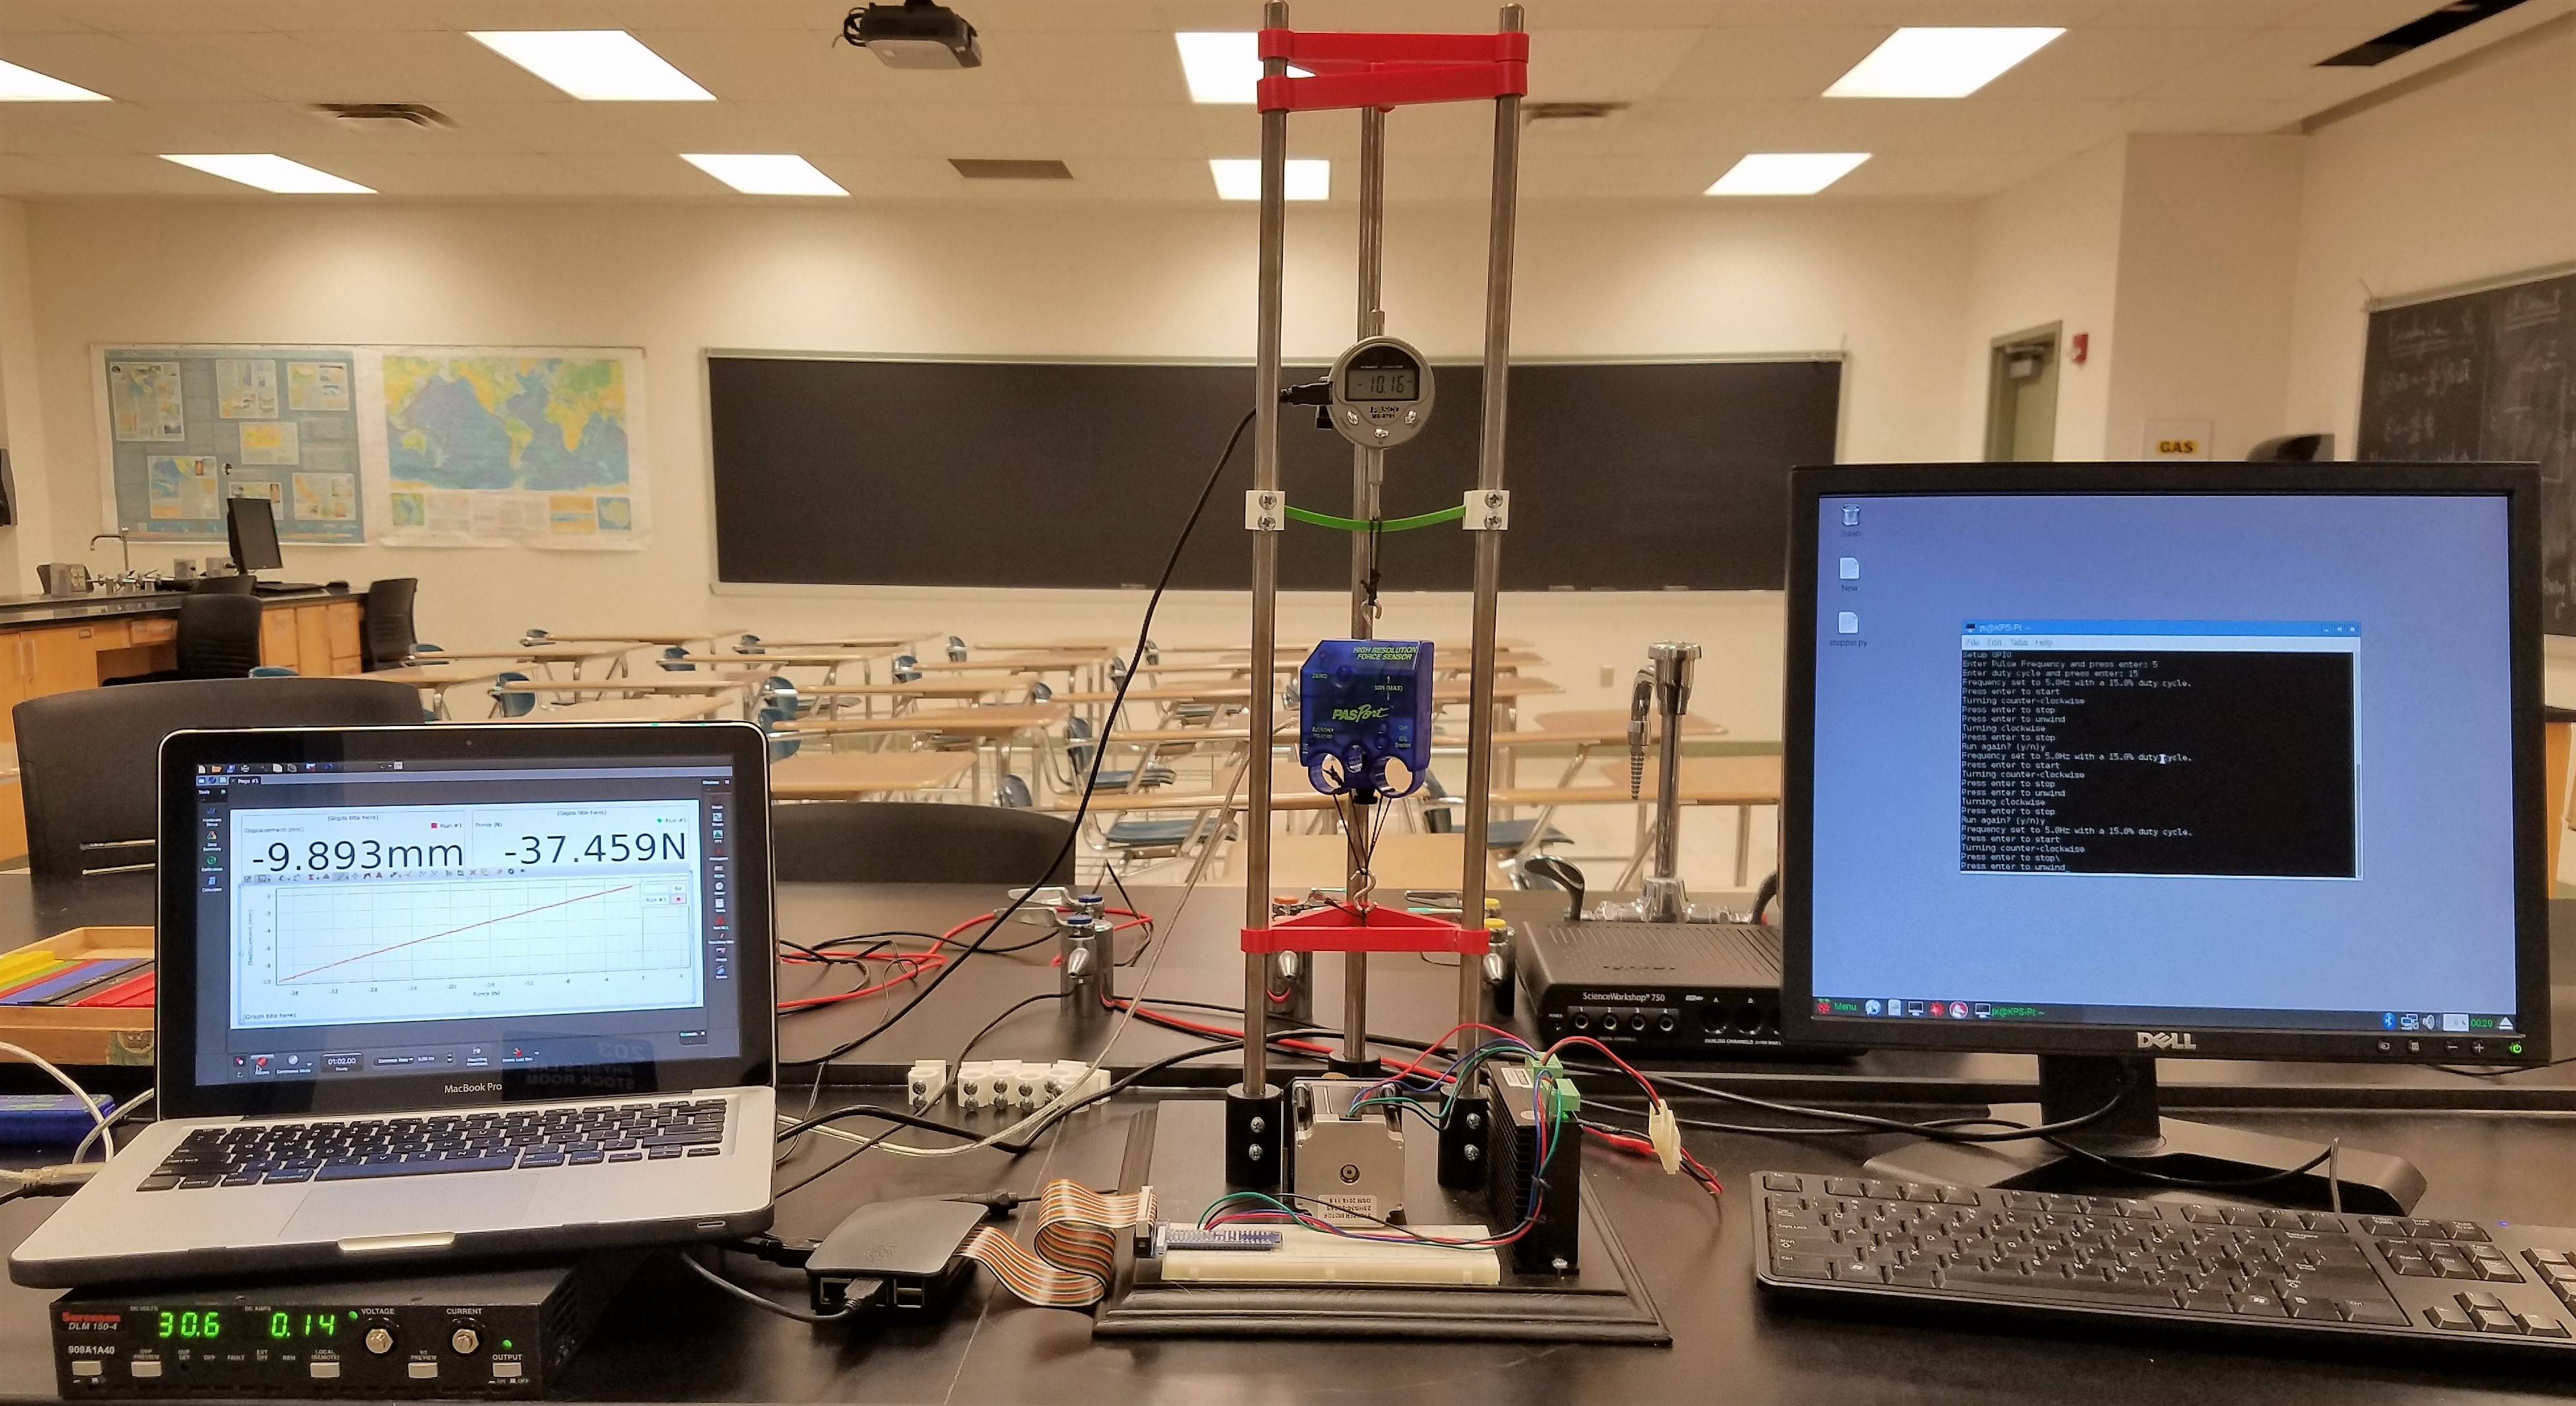
\includegraphics[width=\textwidth]{FIXTURE_SETUP_WHOLE}
	\label{fig:test_fixture}
\end{figure}

All bending tests were conducted using a custom built test fixture. The length of the section to be bent was kept at $120 +0.23/-.033 mm$ for all specimens using a set of custom designed collars (the red components shown in \ref{fig:test_fixture}) to keep the test fixture oriented properly. A NEMA 23 CNC bi-directional stepper motor, model 23HS30-2804S, was used and controlled using a M542T high resolution stepper motor controller at a 1.8\degree step. The motor controller was powered with a Sorensen DLM150-4 power supply at 30V and a maximum of 0.4A and the stepping was controlled using PWM outputs from a Raspberry PI microcomputer (code is attached in Appendix A) at a rate of 5 Hz with a 15\% duty cycle. Non-elongating woven kevlar cord was used to perform the bending tests in order to minimize error caused by deformation of the mechanisms used to apply loading to the test specimen. \par

	PASCO Capstone software was used to record data captured by the PASCO High Resolution Force Sensor (PS-2189) and PASCO Displacement Sensor (PS-2204) at a 5 Hz common rate. The force applied to the specimens started at approximately 1N and was raised to a maximum of 50N, or until a deformation exceeding the measuring capabilities of the deformation gauge was reached.

\subsection{Test Fixture Design}
\begin{figure} [H]
\centering
	\caption{Test Fixture}
	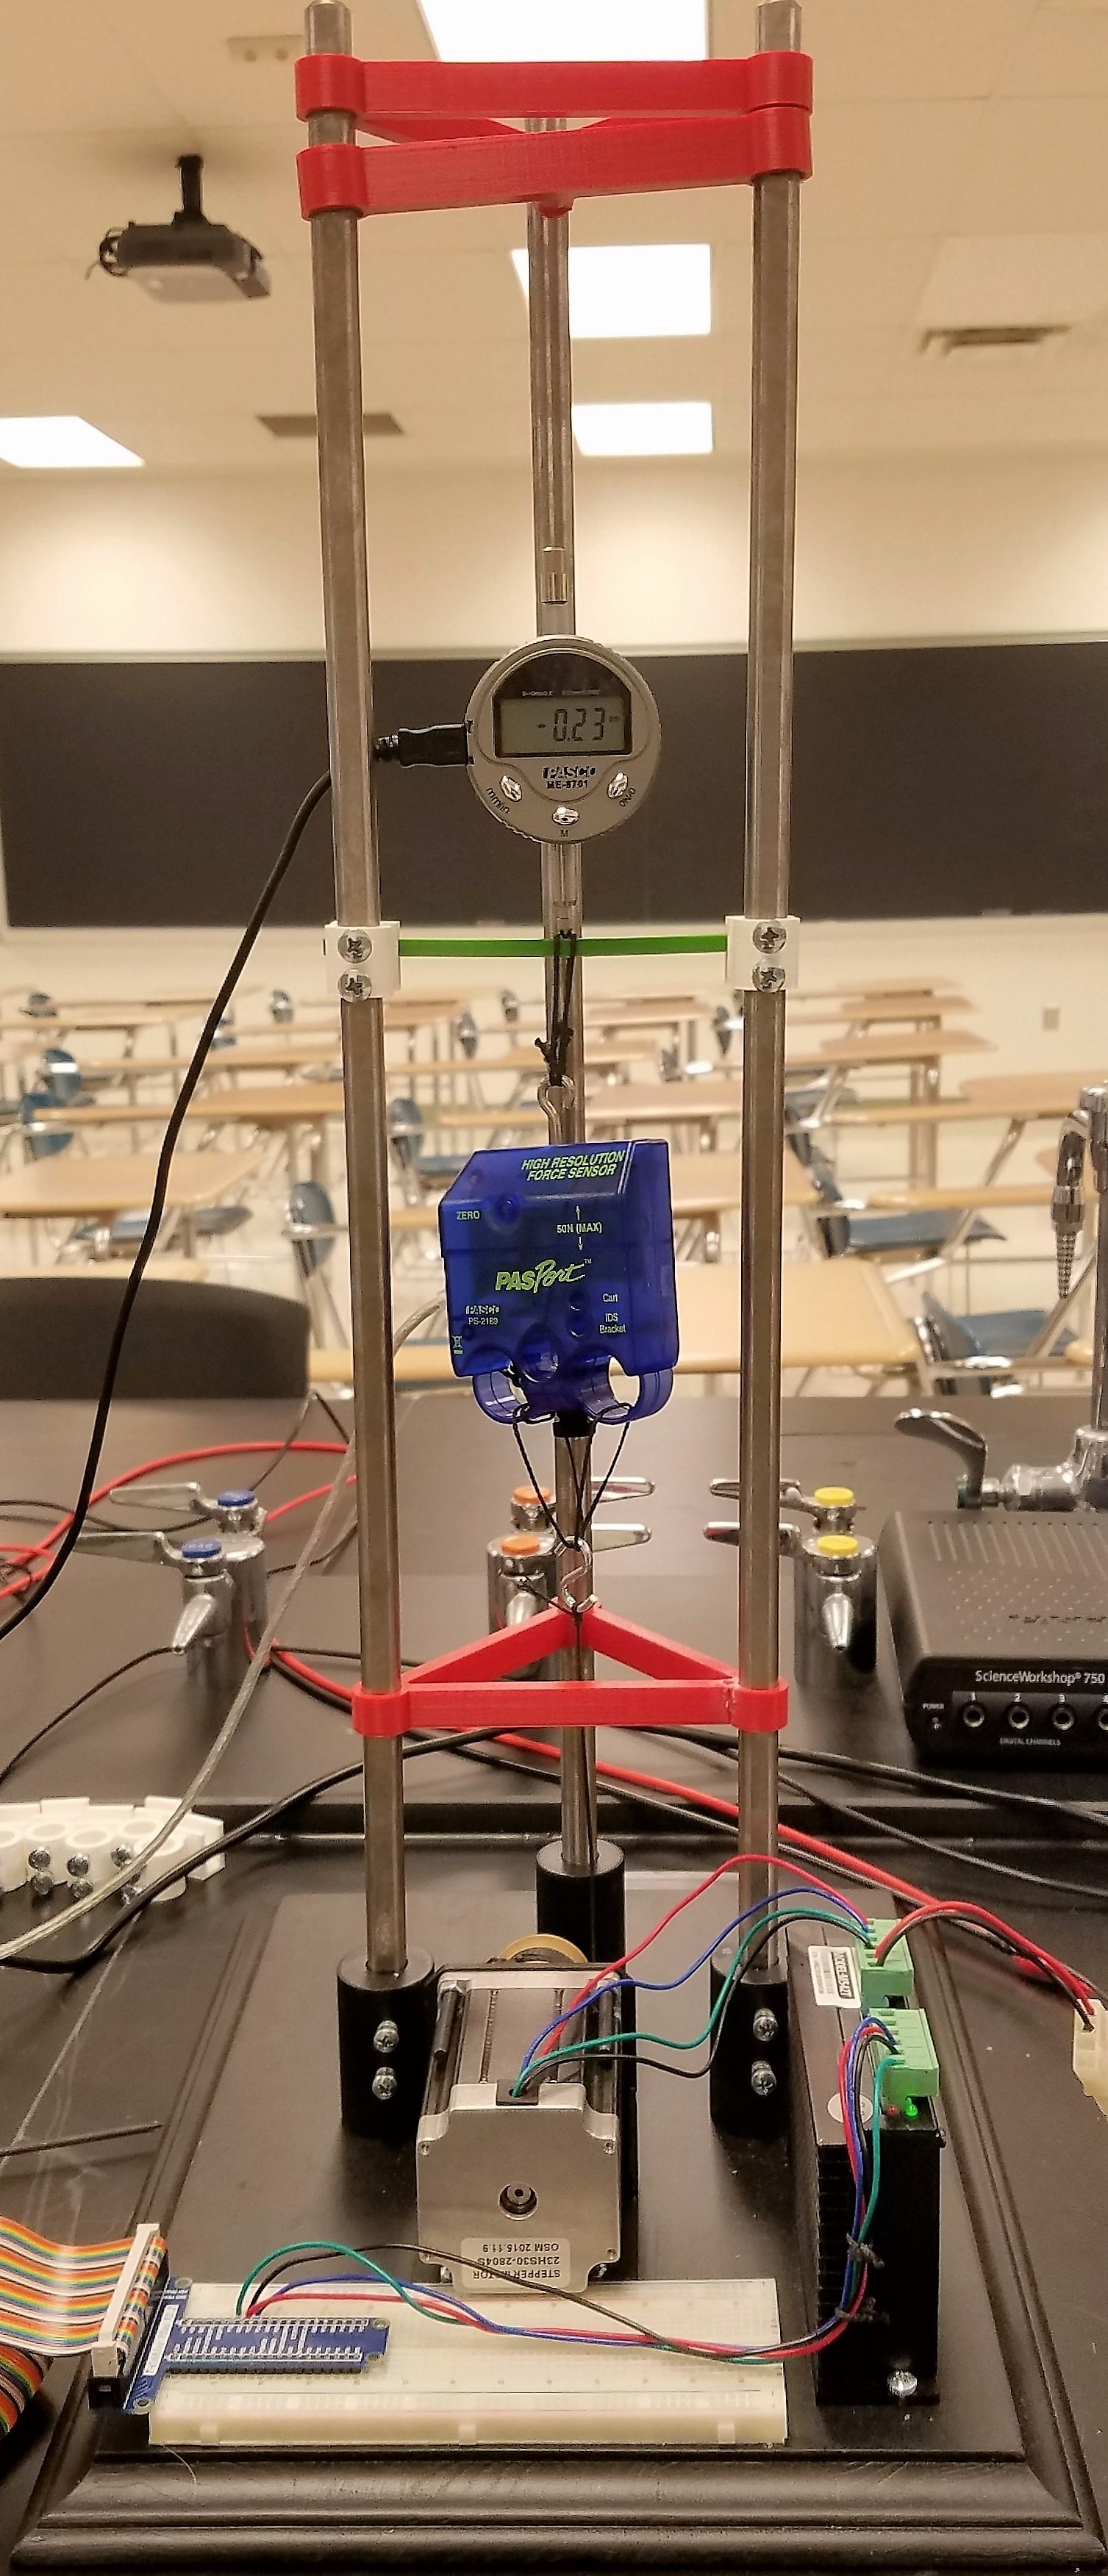
\includegraphics[height=12cm]{FIXTURE_SETUP_DETAIL}
	\label{fig:test_fixture_detail}
\end{figure}

\par
The test fixture in figure \ref{fig:test_fixture_detail} was designed in order to have a bending length $L$ from \ref{eq:modulus} of 120mm. The bending fixtures were created in Solidworks as detailed by the drawing (figure \ref{fig:Bend_Point_Dwg})and were designed to fit the specimens based on measured sizes with minimal tolerance for movement in order to keep the application of force constant throughout the bending tests. Dimension A figure \ref{fig:Bend_Point_Dwg} was set to 5.4mm, 8.2mm, 11.6mm, 15.2mm, to accommodate the different sizes of beams. The center of this bending structure was kept constant in order to provide a bend point 22mm in front of the center of the d-profile rod these fixtures were mounted on. Figure \ref{fig:Bend_Points} shows the printed bend point structures.\par

\begin{figure} [H]
\centering
	\caption{Dimensions of Bend Points}
	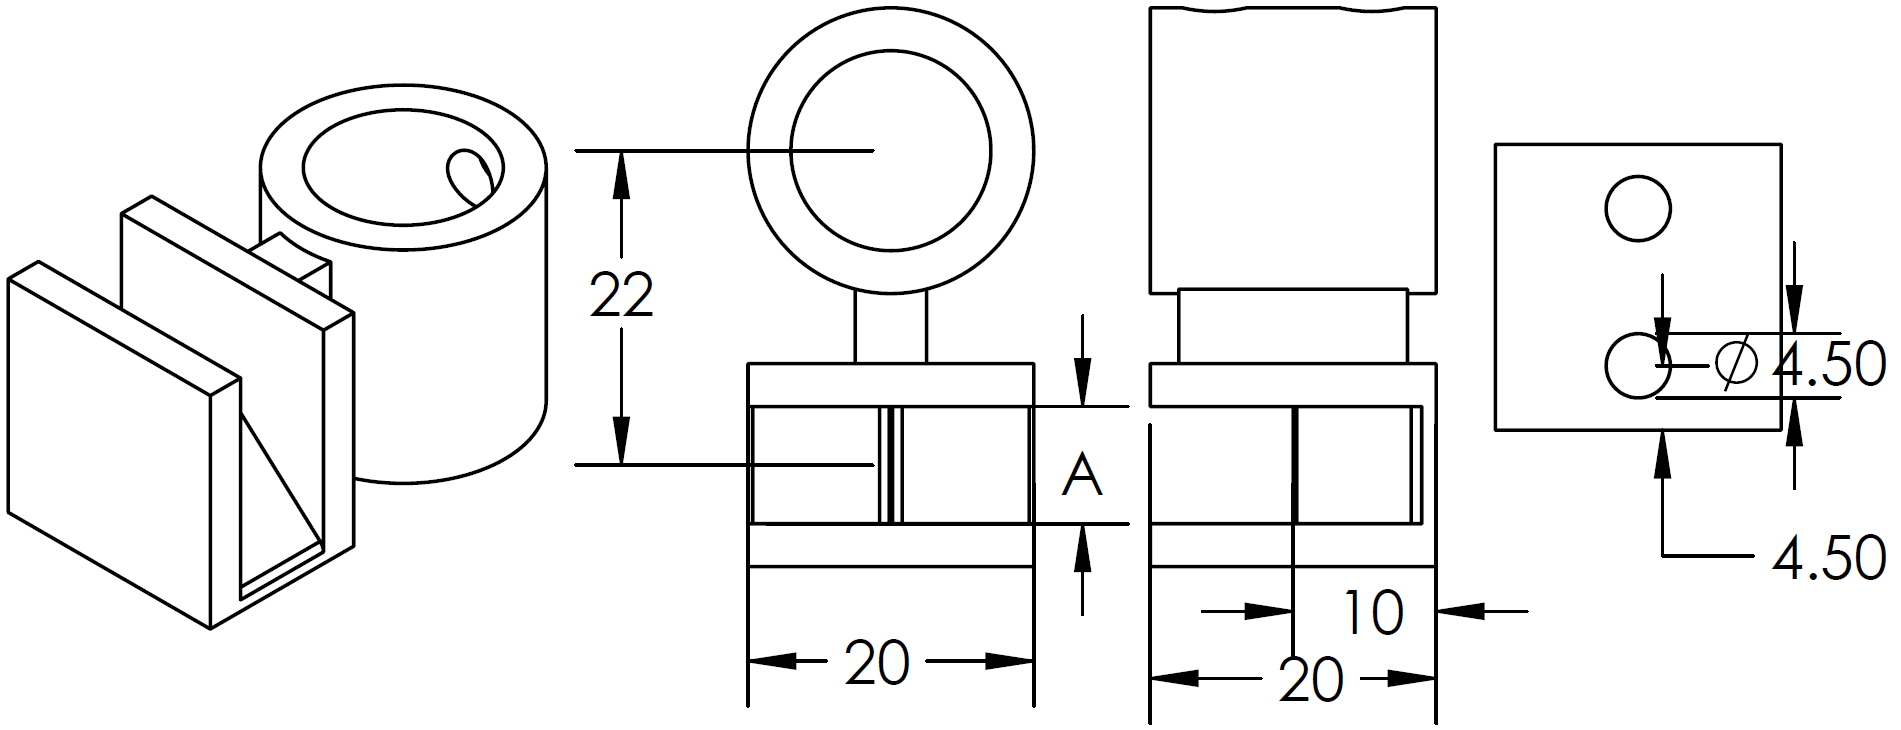
\includegraphics[width=\textwidth]{Bend_Point_DWG}
	\label{fig:Bend_Point_Dwg}
\end{figure}


\begin{figure} [H]
\centering
	\caption{Side View of Fixture Bend Points}
	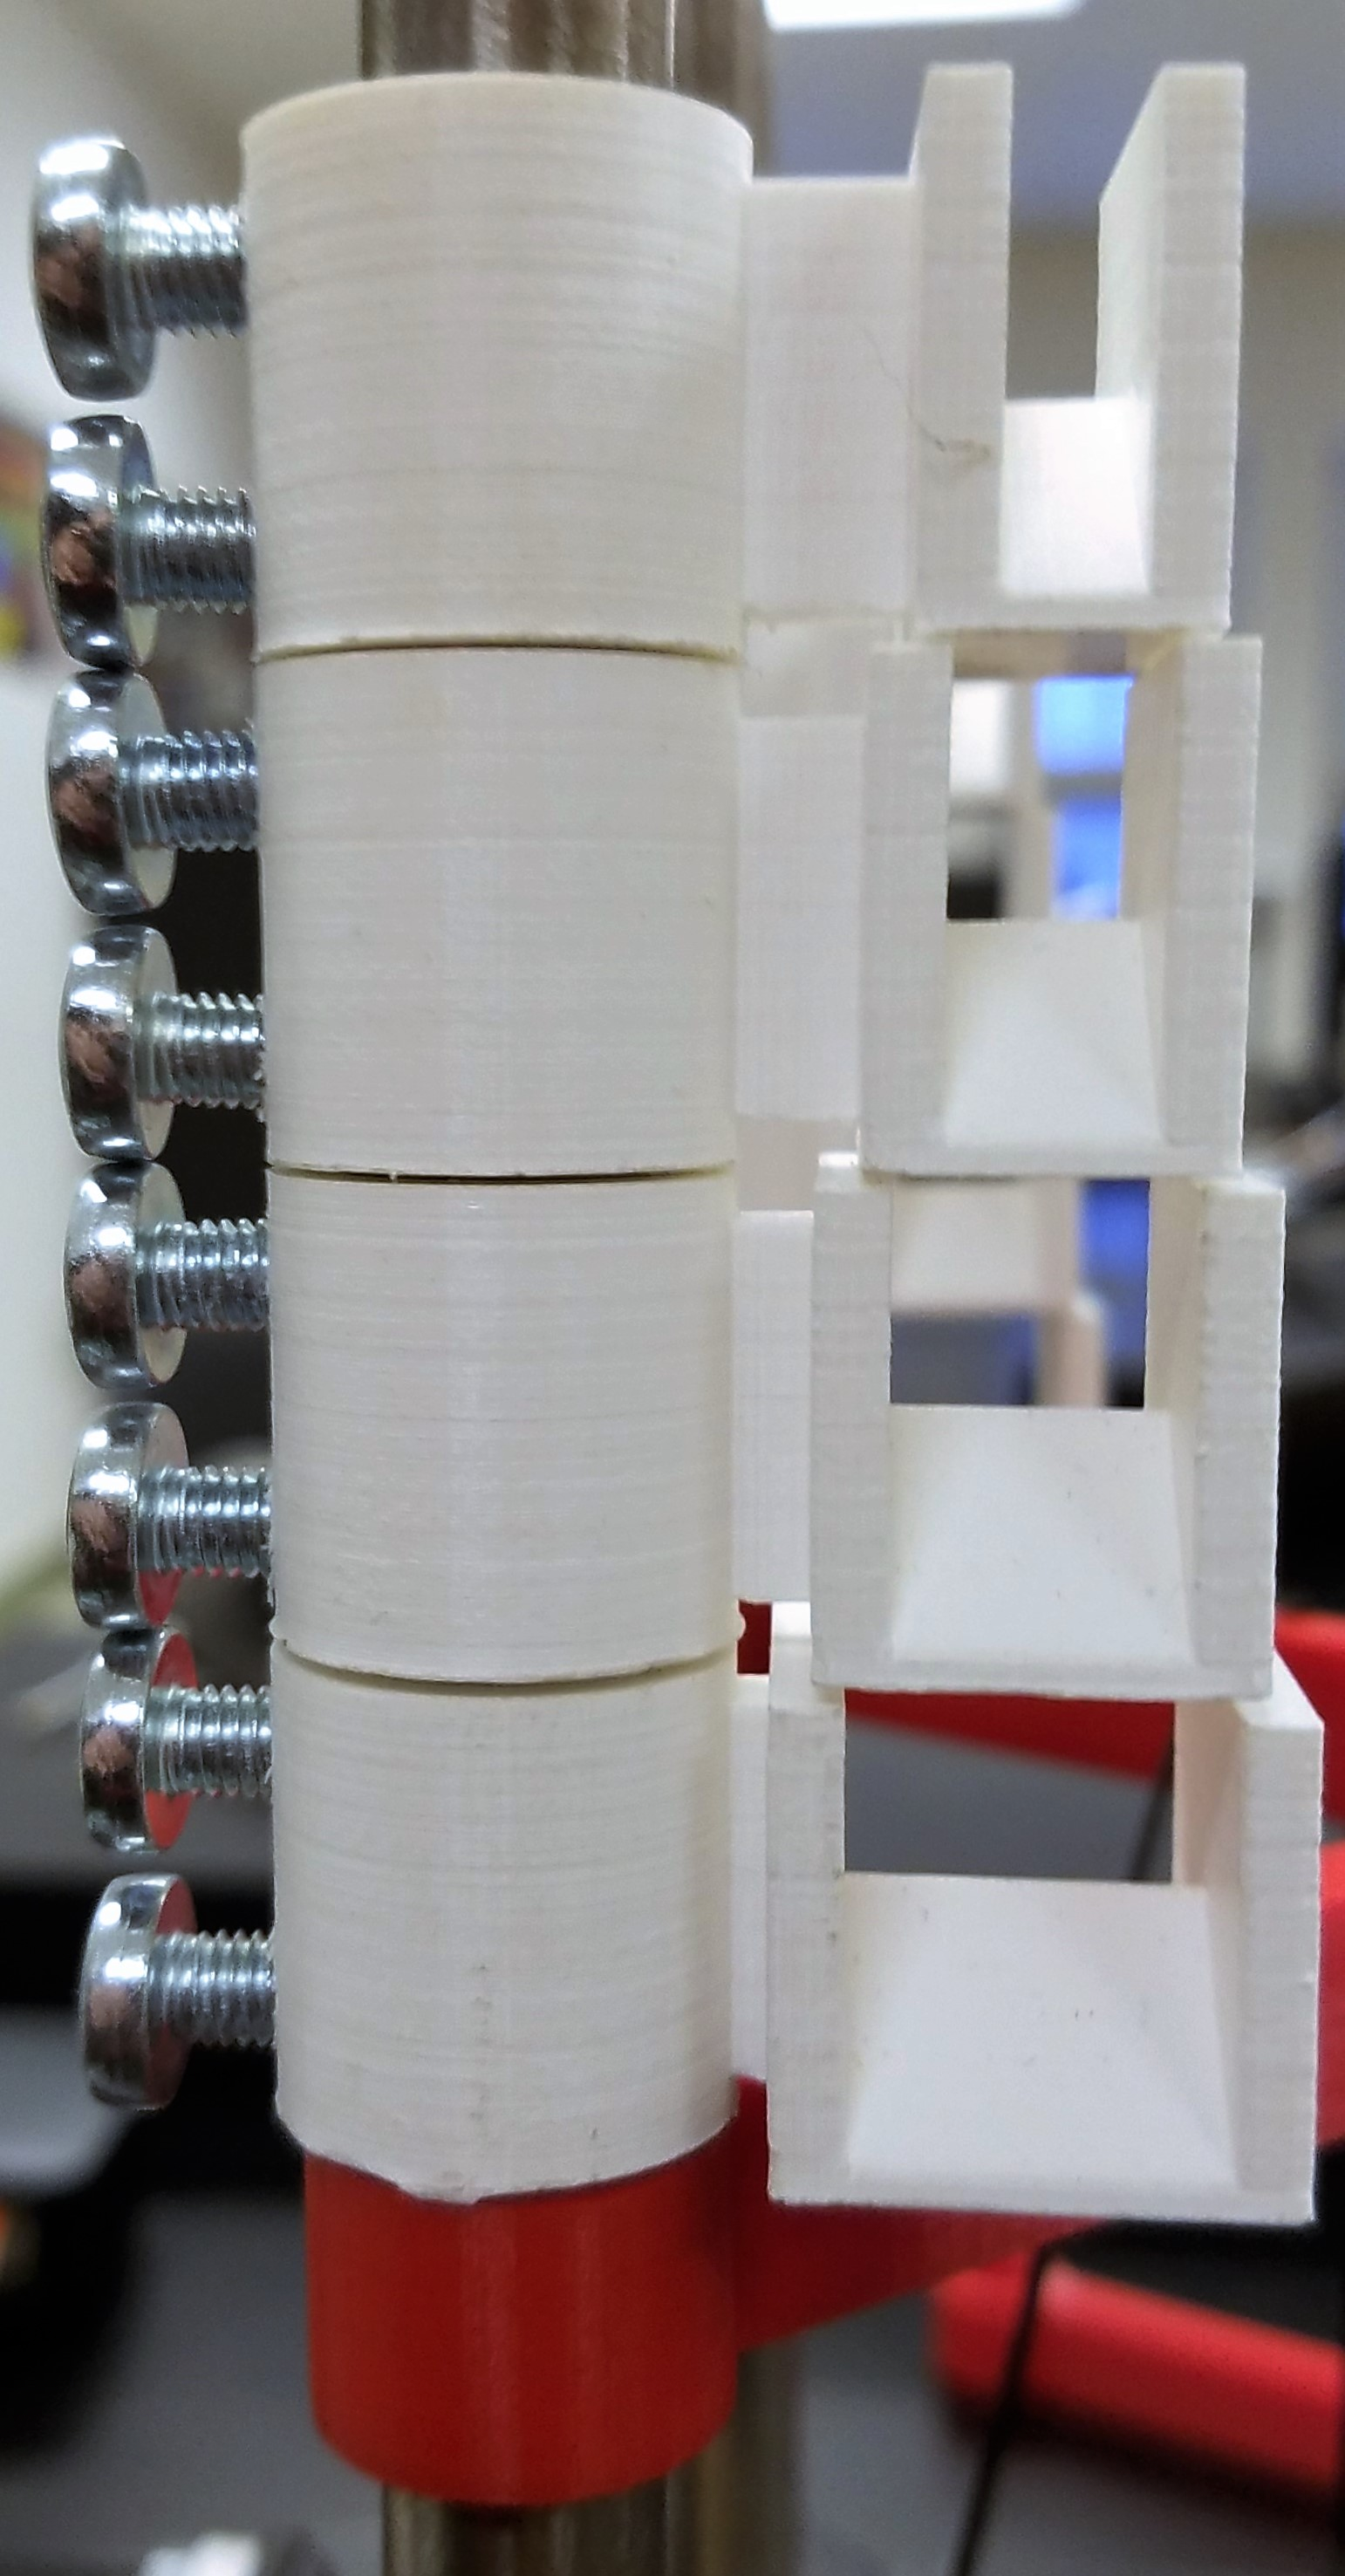
\includegraphics[height=3in]{FIXTURE_SETUP_BEND_POINTS}
	\label{fig:Bend_Points}
\end{figure}

	The test fixtures were designed to be larger and more robust than the beams printed in order to minimize error in measuring the beam deformation by the test fixtures themselves deforming. All test fixtures were printed 100\% solid and then were tapped for a 5mm screw to hold them in place on the test fixture.


\subsection{Test Specimen Design}
	The test specimens for Phase I were designed with two objectives: To determine the effect of increasing density of infill on the 3D printed objects and to see if the size of an object relative to the wall thickness and infill plays any role in determining the strength of the object. An example of 25\% and 50\% infill are shown in figures \ref{fig:25_PLA} and \ref{fig:50_PLA}, respectively. The beams were designed for each rectangular and square size to have identical cross-sectional area. In the table below, the nominal size of the test specimens are listed.
	\begin{table} [H]
		\centering
		\begin{tabular}{ l l l }
		\noalign{\hrule height 2pt}
		Size & Square & Rectangular \\ \hline
		100\% & 5.17x5.17 & 7.53x3.6 \\
		150\% & 7.75x7.75 & 11.3x5.4 \\
		200\% & 10.34x10.34 & 15.06x7.2 \\ \hline
		\multicolumn{3}{c}{Materials} \\ \hline
		ABS & PLA \\ \hline
		\multicolumn{3}{c}{Fill Percentage} \\ \hline
		\multicolumn{3}{c}{20\%} \\
		\multicolumn{3}{c}{50\%} \\
		\multicolumn{3}{c}{100\%} \\ \hline
		\end{tabular}
		\caption{List of Plastic Beam Specimens}
		\label{tab:BeamFab}
	\end{table}

	The measurements for the test specimens were taken at each end and the midpoint of each beam and averaged; this data is available in Appendices B \& C. Table \ref{tab:BeamComp} below shows the average of each set of specimen sizes as well as the deviation from the nominal value. The largest deviation was in the height of the small rectangular samples at 2.78\% deviation from the nominal value listed in Table \ref{tab:BeamFab}.
	
	\begin{figure} [H]
		\centering
		\caption{Printing 25\% Fill PLA Test Specimens}
		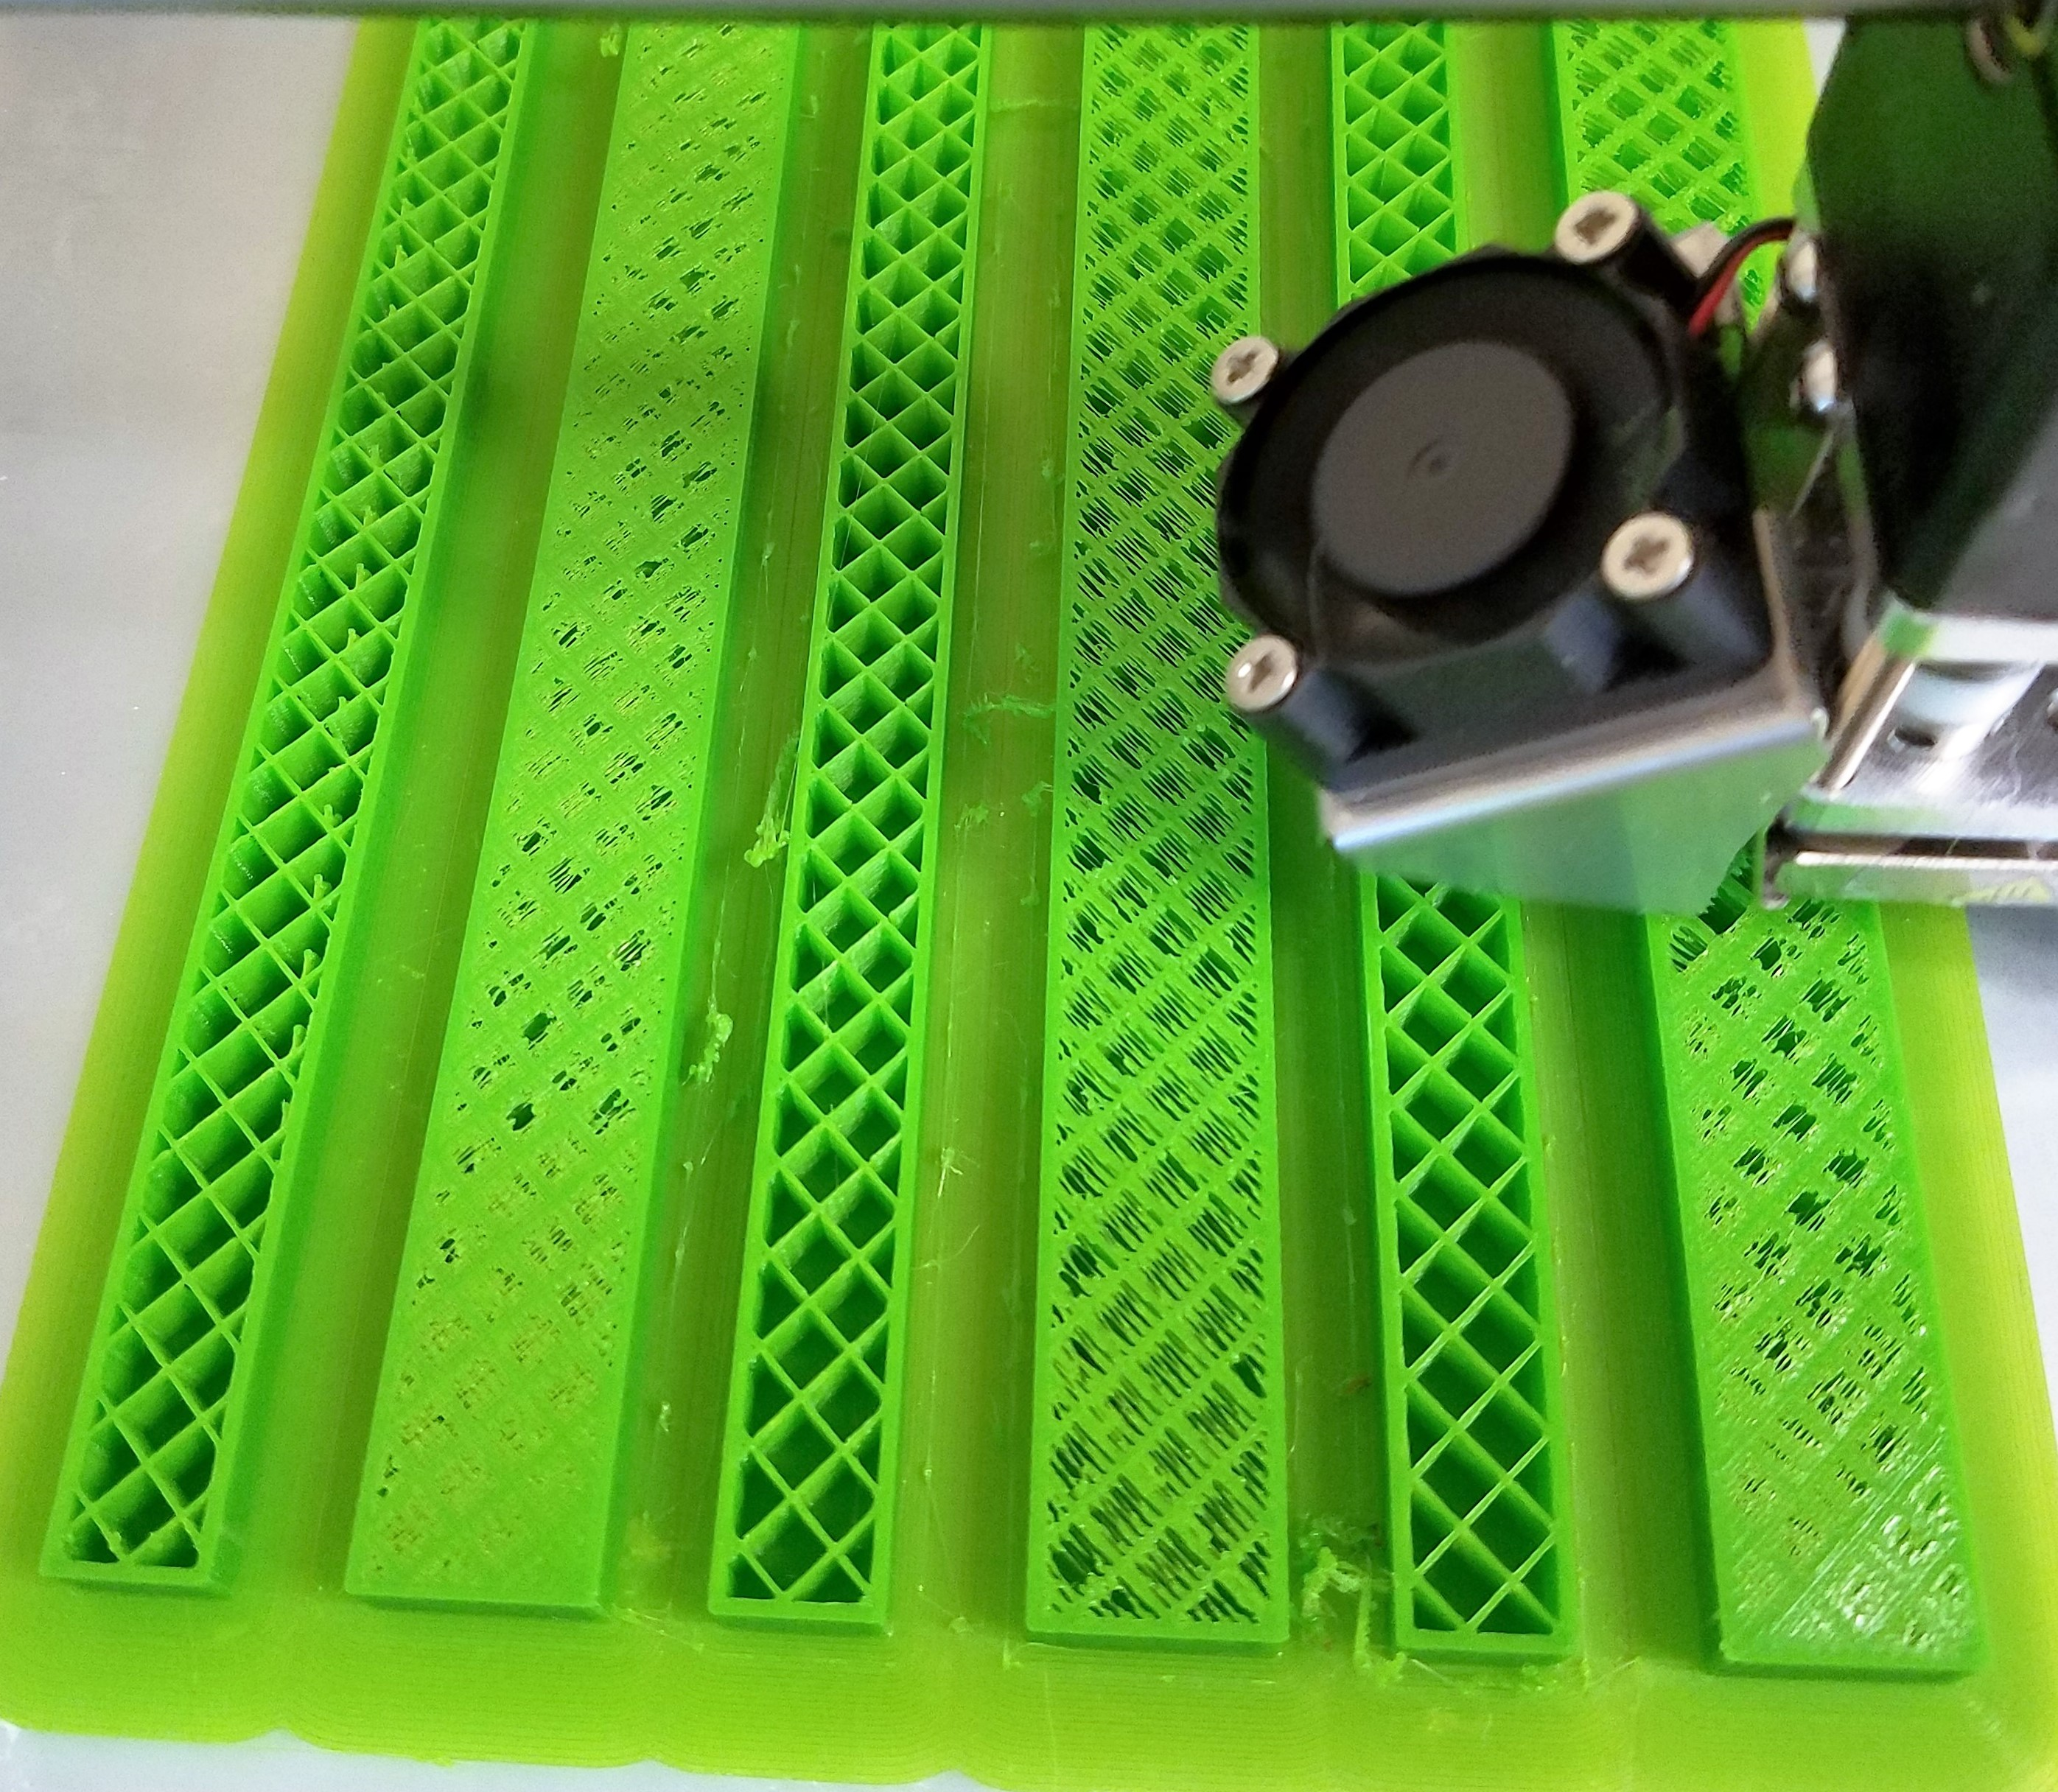
\includegraphics[width=.75\textwidth]{Printer_PLA_Beams_2}
		\label{fig:25_PLA}
	\end{figure}
	
	\begin{table} [h]
		\centering
		\begin{tabularx}{\textwidth}{  X  X  X  X  X  }
		\noalign{\hrule height 2pt}
			& Width (mm) & Height (mm) & Width Deviation (\%) & Height Deviation (\%) \\ \hline
			Square Size 1 & 5.24 & 5.18 & 1.35 & 0.19 \\ 
			Square Size 2 & 7.74 & 7.8 & 0.13 & 0.65 \\ 
			Square Size 3 & 10.25 & 10.34 & 0.87 & 0 \\ \hline
			Rectangle Size 1 & 7.65 & 3.5 & 1.59 & 2.78 \\ 
			Rectangle Size 2 & 11.33 & 5.3 & 0.27 & 1.85 \\ 
			Rectangle Size 3 & 14.98 & 7.12 & 0.53 & 1.11 \\ \hline
		\end{tabularx}
		\caption{List of Plastic Beam Measurements \& Deviation}
		\label{tab:BeamComp}
	\end{table}
	
	\begin{figure} [H]
		\centering
		\caption{Printing 50\% Fill PLA Test Specimens}
		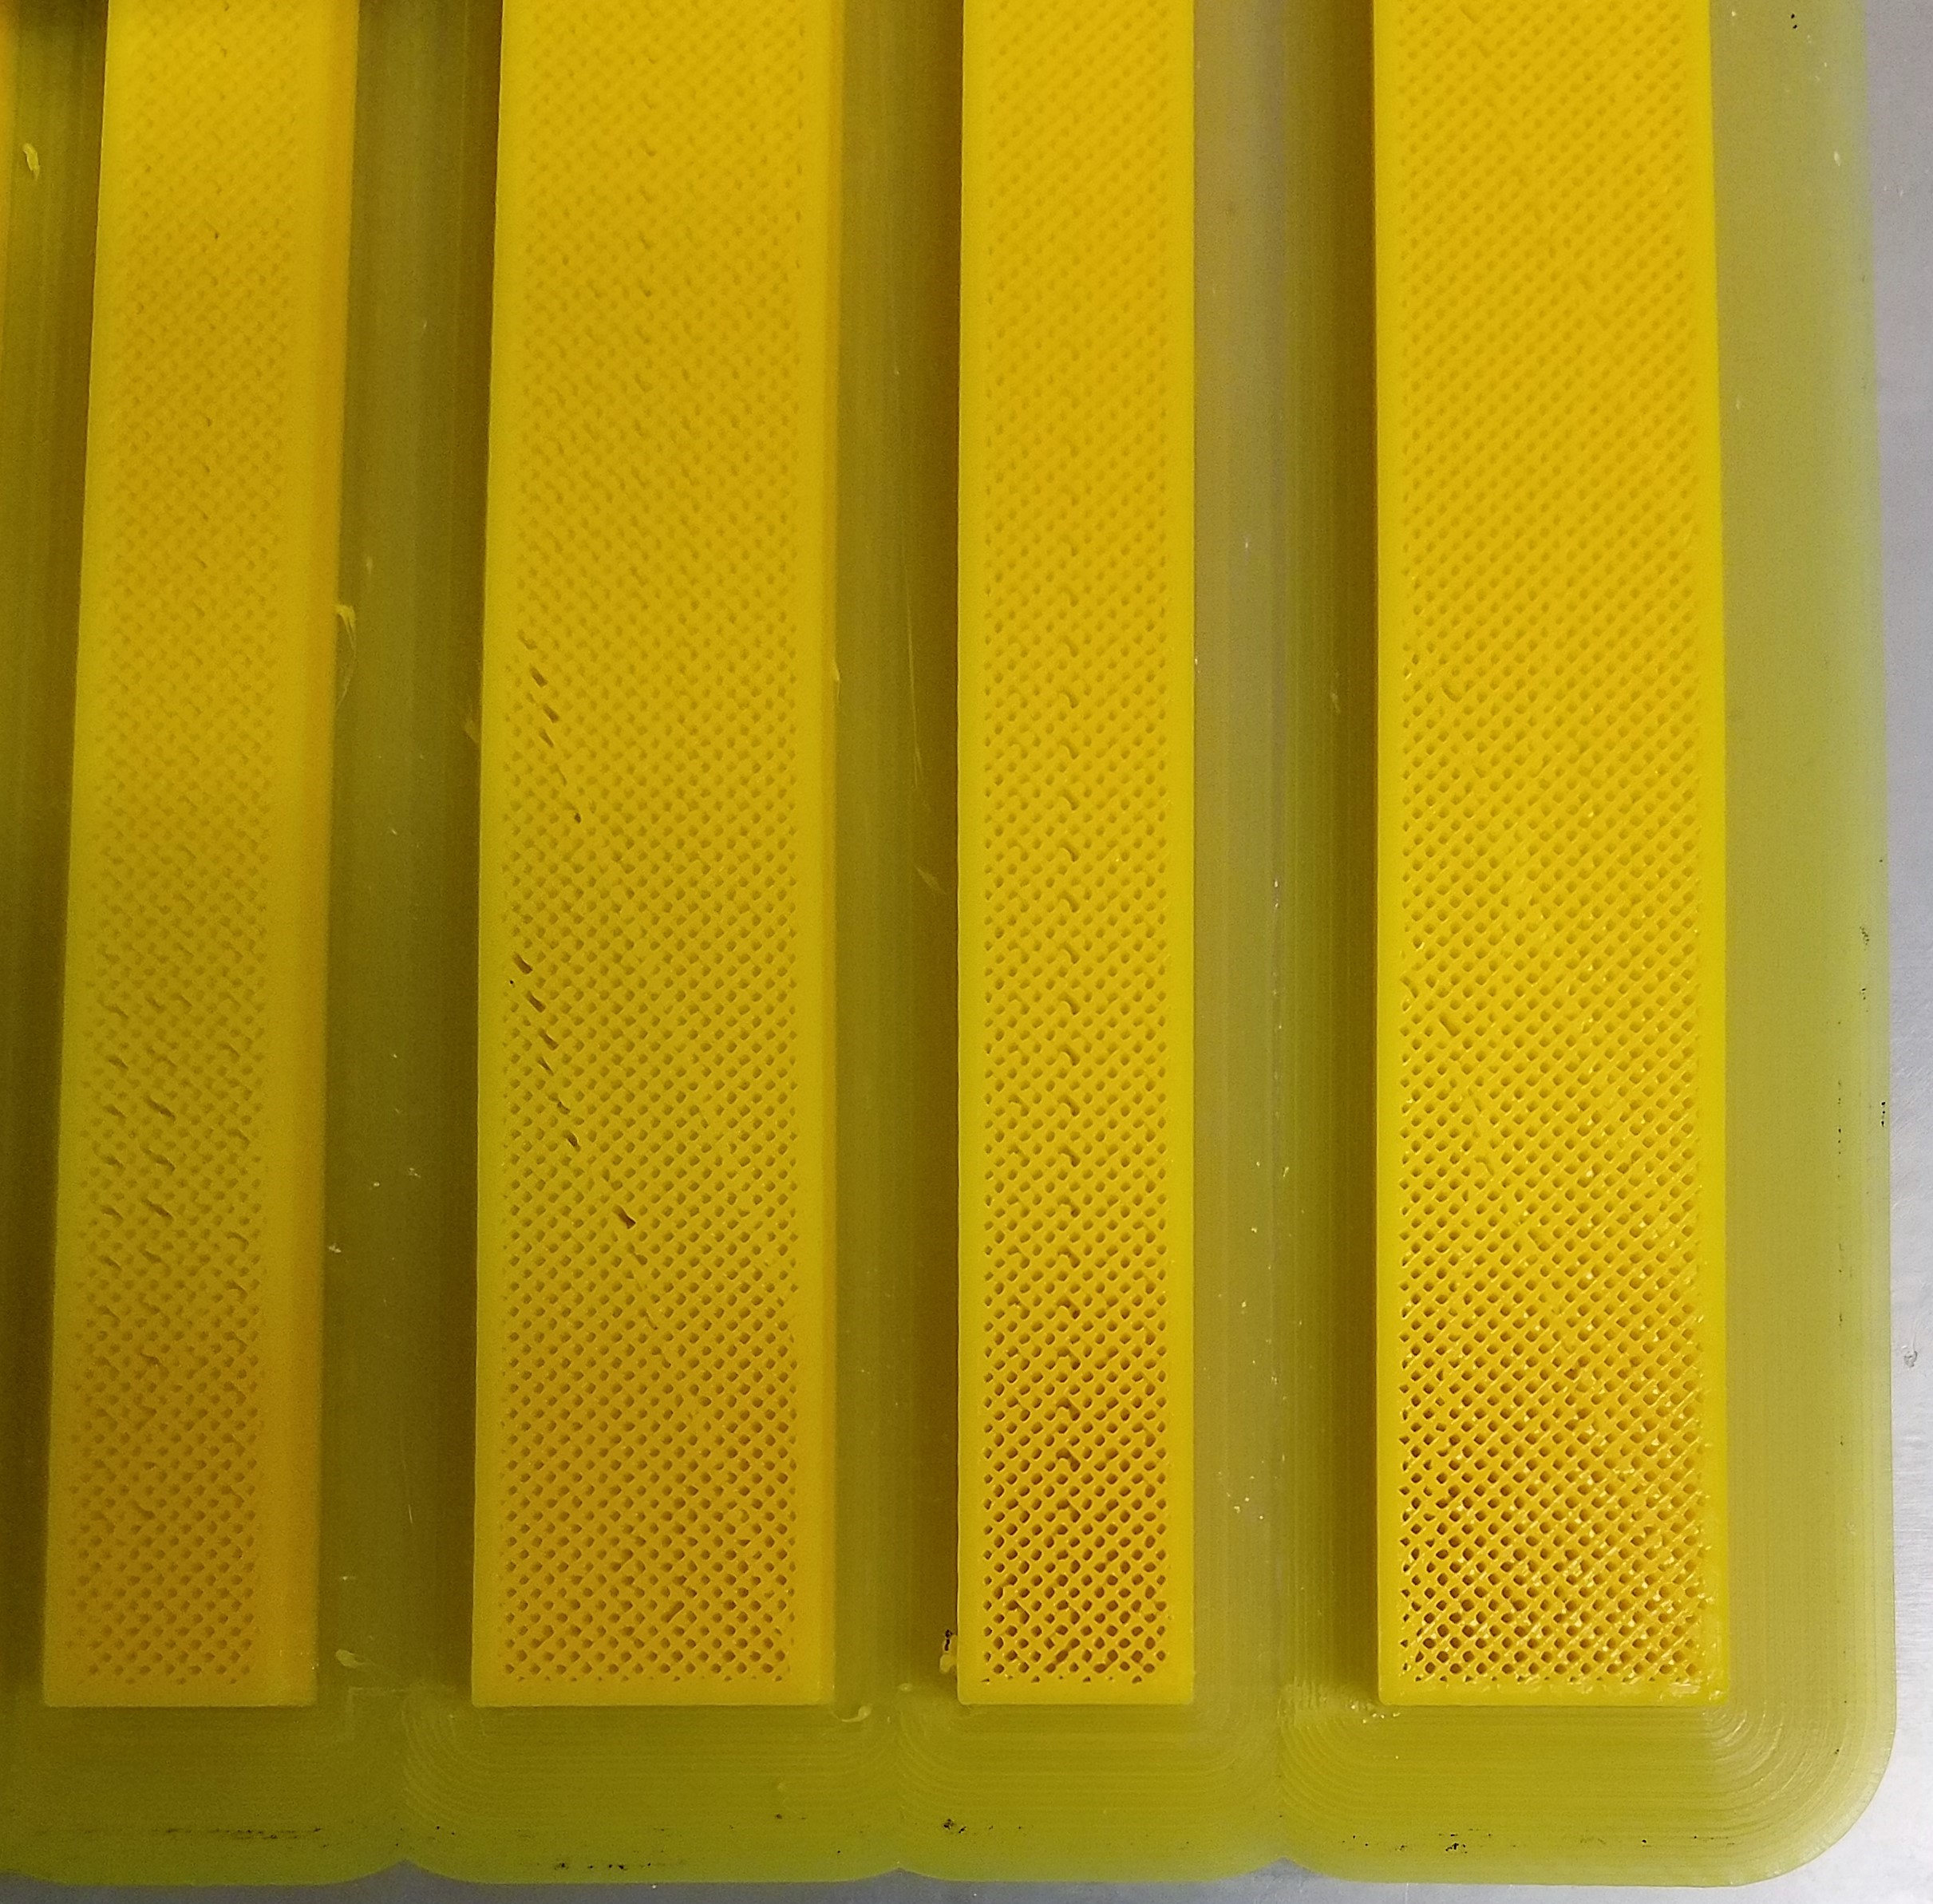
\includegraphics[width=.75\textwidth]{Printer_PLA_Beams_4}
		\label{fig:50_PLA}
	\end{figure}
		
\subsection{Examining Elastic Moduli}
	The Elastic Modulus of each specimen was obtained by using formula \ref{eq:modulus} for each data point and averaging the data for the linear elastic region. From this calculated modulus, an estimated force for deflection within the linear elastic region was determined and then compared to the actual value from experimentation. This uncertainty in the ability to calculate the force at a given deflection, which is similar to the focus of Adamczak, et al., was investigated for all specimens. \citep{Adamczak2014} 
	
	Table \ref{tab:PLAModAvg} details the average of the Modulus of Elasticity and Uncertainty for all 3 samples of each in-fill level of the rectangular and square PLA specimens. The following graphs in figures \ref{fig:PLA_Modulus} \& \ref{fig:PLA_Uncertainty} illustrate the data for the PLA test specimens. Detailed data can be found in appendices B \& C.
	
	\begin{table} [h]
		\centering	
		\begin{tabularx}{\textwidth}{ X X X }
		\noalign{\hrule height 2pt}
			\multicolumn{3}{c}{PLA Modulus of Elasticity Averages} \\ \hline
			SAMPLE & AVG MODULUS (GPa) & UNCERTAINTY (\%) \\ \hline
			SQUARE 25\% & 2.425 & 4.859 \\ 
			SQUARE 50\% & 2.377 & 1.903 \\ 
			SQUARE 100\% & 3.33 & 1.833 \\ 
			RECTANGLE 25\% & 2.419 & 1.712 \\ 
			RECTANGLE 50\% & 2.66 & 1.524 \\ 
			RECTANGLE 100\% & 3.146 & 1.178 \\ \hline
			AVERAGES & 2.726 & 2.168 \\ \hline
		\end{tabularx}
		\caption{Average PLA Beam Specimen Moduli of Elasticity}
		\label{tab:PLAModAvg}
	\end{table}
	
	\begin{figure} [H]
		\centering
		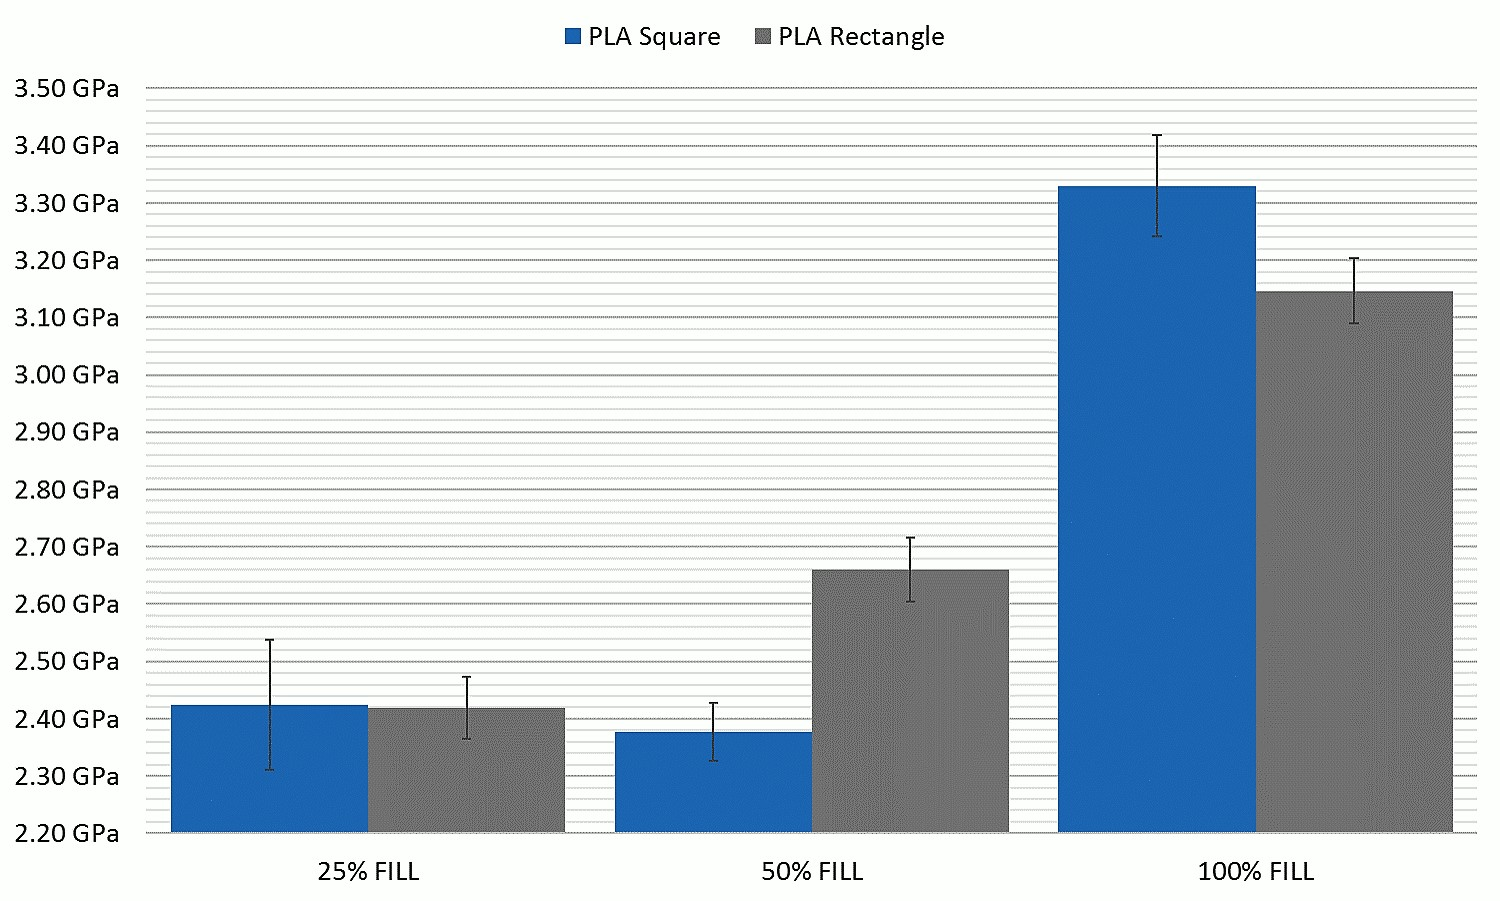
\includegraphics[width=\textwidth]{CHART_PLA_Elasticity}
		\caption{Average PLA Modulus of Elasticity (GPa)}
		\label{fig:PLA_Modulus}
	\end{figure}
	
	\begin{figure} [H]
		\centering
		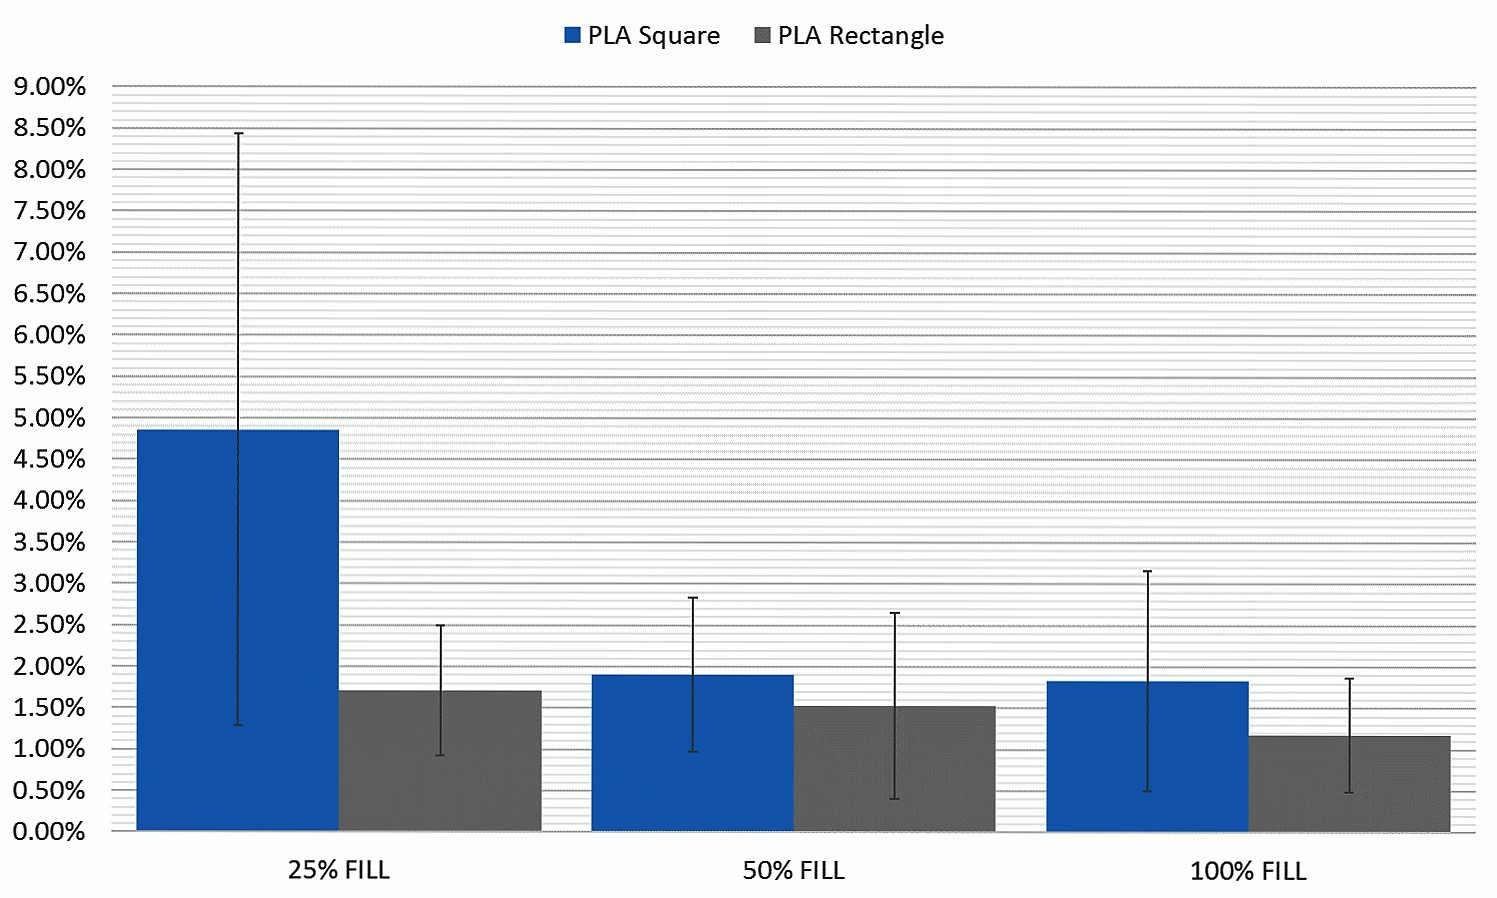
\includegraphics[width=\textwidth]{CHART_PLA_Uncertainty}
		\caption{PLA Uncertainty (\%)}
		\label{fig:PLA_Uncertainty}
	\end{figure}
Similar to table \ref{tab:PLAModAvg}, table \ref{tab:ABSModAvg} contains data for the ABS specimens and the following figures \ref{fig:ABS_Modulus} and \ref{fig:ABS_Uncertanty} illustrate the data for the ABS specimens found in the Appendicies. Of note, ABS Rectangular Specimen \#6 delaminated during testing due to a manufacturing defect, pictured below in figures \ref{fig:Damage1} and \ref{fig:Damage2}.

	\begin{figure} [H]
		\centering
		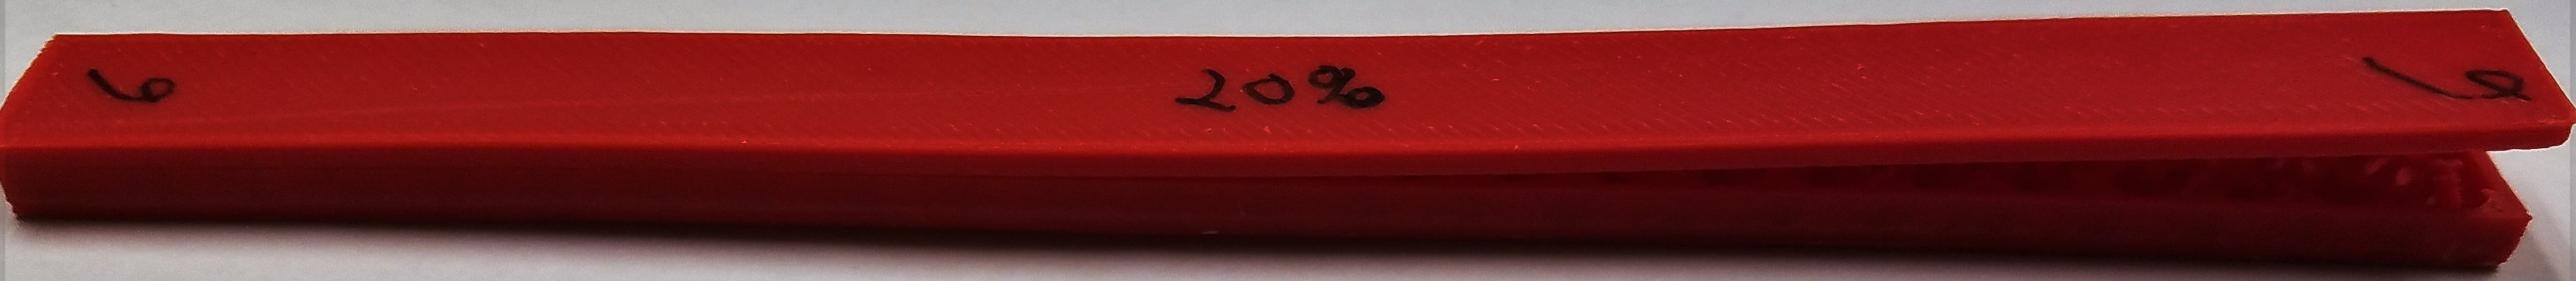
\includegraphics[width=\textwidth]{Damaged_specimen_1}
		\caption{Damaged Specimen Isometric View}
		\label{fig:Damage1}
	\end{figure}
	\begin{figure} [H]
		\centering
		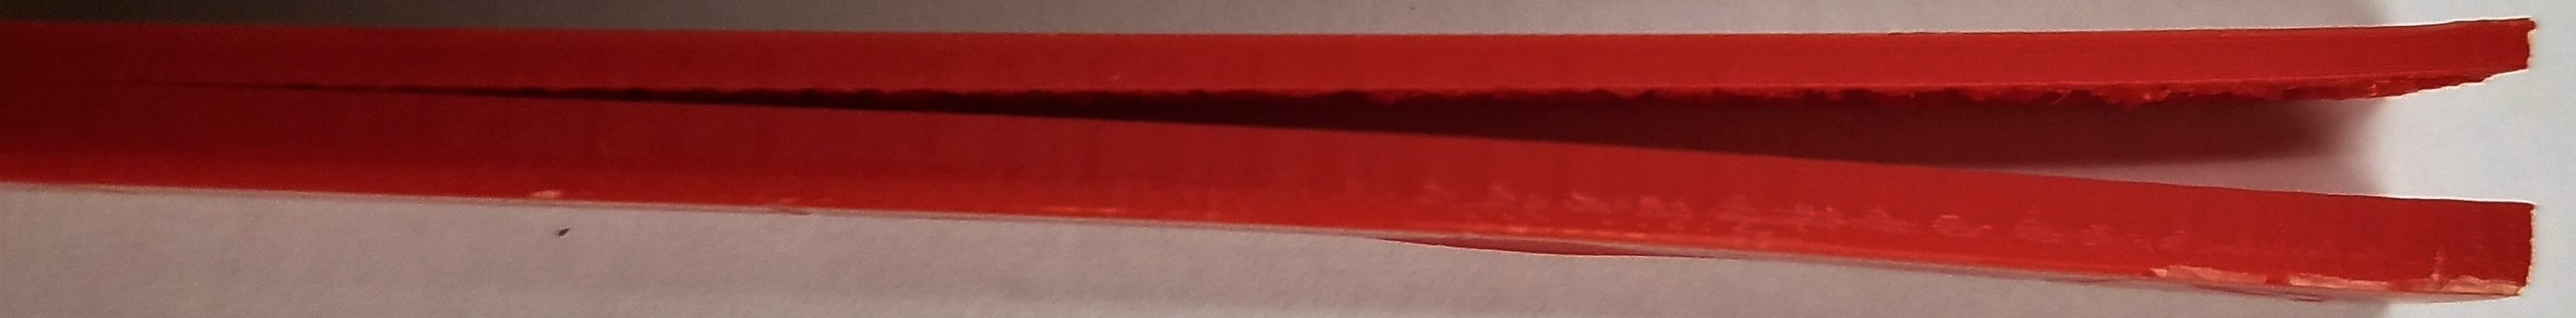
\includegraphics[width=\textwidth]{Damaged_specimen_2}
		\caption{Damaged Specimen Side View}
		\label{fig:Damage2}
	\end{figure}

	\begin{table} [h]
		\centering	
		\begin{tabularx}{\textwidth}{ X X X }
		\noalign{\hrule height 2pt}
			\multicolumn{3}{c}{ABS Modulus of Elasticity Averages} \\ \hline
			SAMPLE & AVG MODULUS (GPa) & UNCERTAINTY (\%) \\ \hline
			SQUARE 25\% & 1.268 & 1.117 \\ 
			SQUARE 50\% & 1.418 & 1.309 \\ 
			SQUARE 100\% & 1.946 & 1.627 \\ 
			RECTANGLE 25\% & 1.439 & 1.282 \\ 
			RECTANGLE 50\% & 1.596 & 1.172 \\ 
			RECTANGLE 100\% & 1.917 & 1.395 \\ \hline
			AVERAGES & 1.597 & 1.317 \\ \hline
		\end{tabularx}
		\caption{Average ABS Beam Specimen Moduli of Elasticity}
		\label{tab:ABSModAvg}
	\end{table}

	\begin{figure} [H]
		\centering
		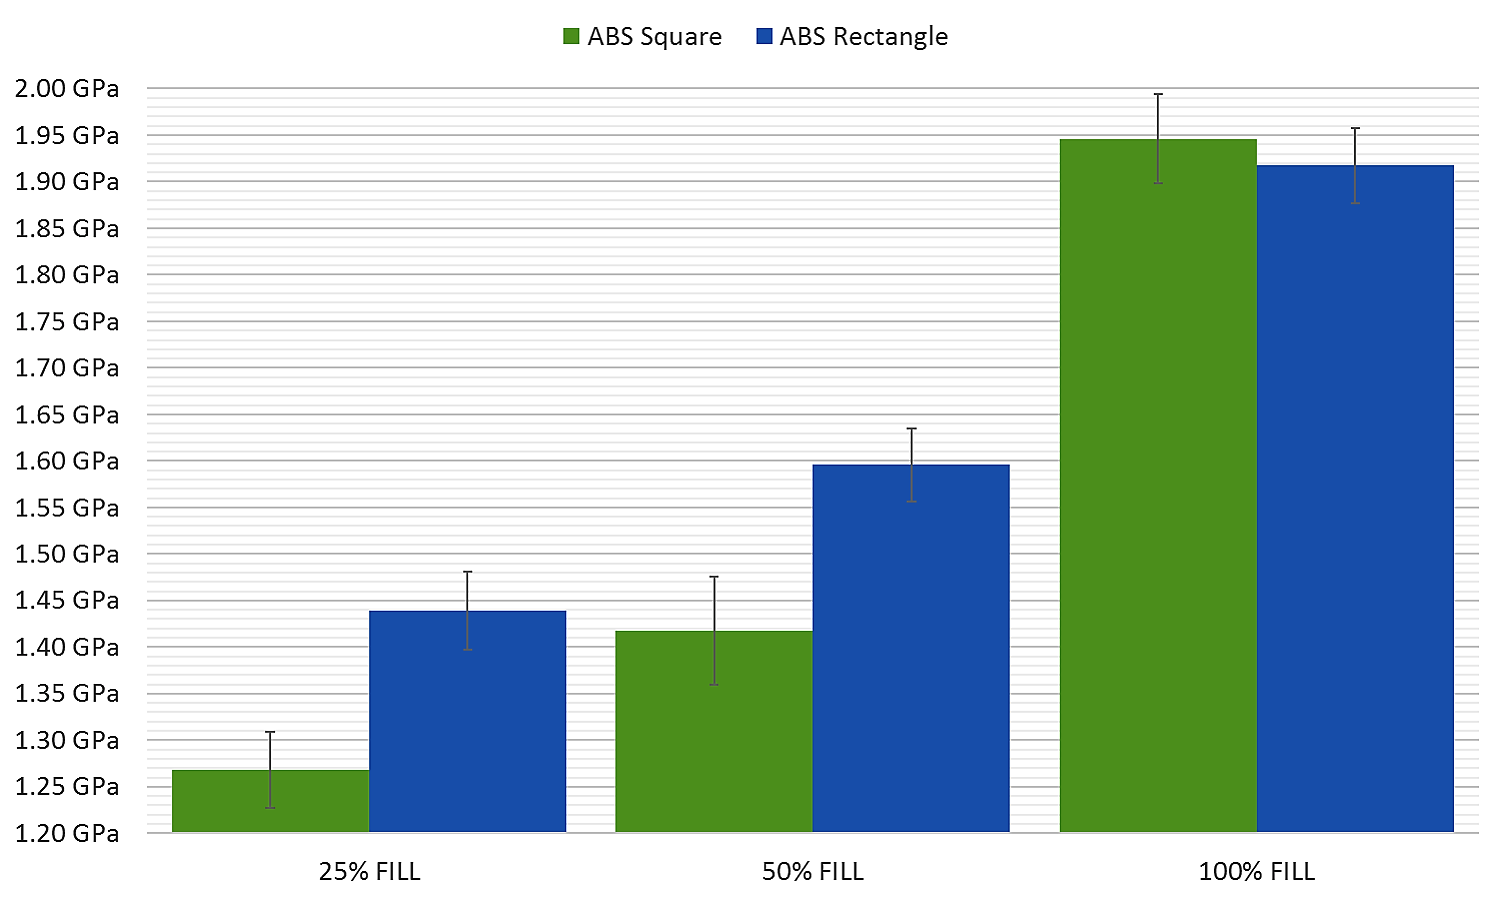
\includegraphics[width=\textwidth]{CHART_ABS_Elasticity}
		\caption{Average ABS Modulus of Elasticity (GPa)}
		\label{fig:ABS_Modulus}
	\end{figure}
	
	\begin{figure} [H]
		\centering
		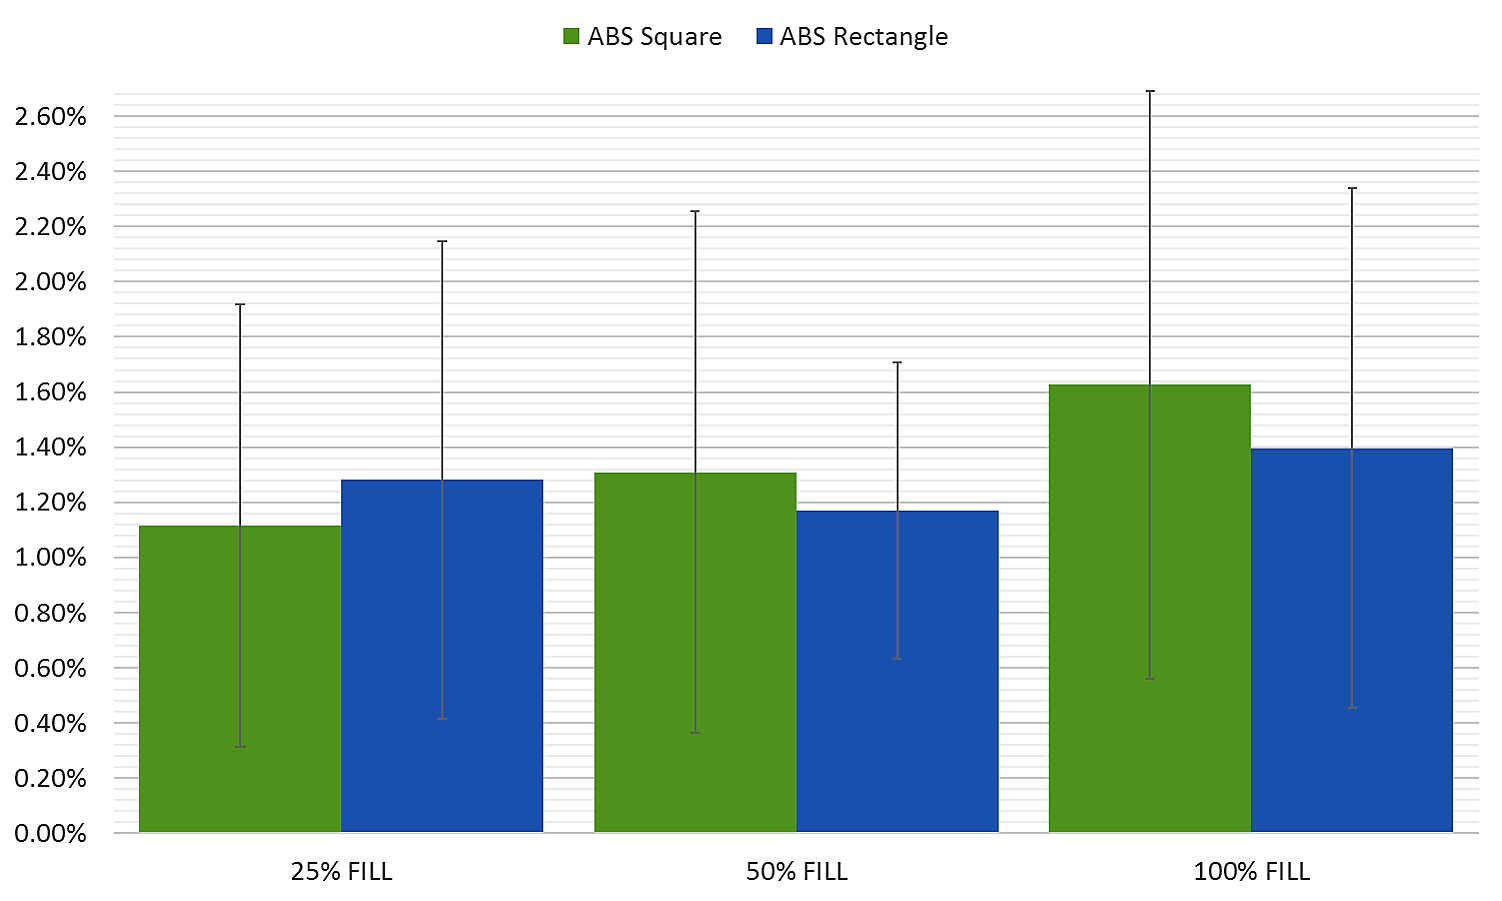
\includegraphics[width=\textwidth]{CHART_ABS_Uncertainty}
		\caption{ABS Uncertainty (\%)}
		\label{fig:ABS_Uncertanty}
	\end{figure}
	
	The experimental data was compared to values found in the literature. As reported in table \ref{tab:PerezABS}, Perez determined the Modulus of Elasticity of the ABS test specimens to be about 1.53 GPa for the specimens printed with their layers oriented parallel to the direction of loading \citep{TorradoPerez2014}. The average modulus of 1.597 GPa found experimentally shows an approximate 4.4\% difference from the ABS modulus reported in the covered literature.
	
	As for the modulus of the PLA specimens, our determined modulus is 2.726 GPa, compared to the 2.159 GPa found by Wendt, et al., noted in table \ref{tab:WendtPLAS} \citep{Wendt2015}. This $\approx 21\%$ difference is most likely due to the fact that Wendt tested single layer specimens as opposed to multi-layer, as well as defects in manufacturing. The single layer specimens were most likely more susceptible to stress concentration due to defects compared to the multi-layer specimens as the printer rotates the orientation of layers as it prints. For example, the first layer may be printed completely in the Y direction while the second layer is at a 45 degree angle to the X and Y axis. This rotation of layers most likely adds to the strength of the objects.

\subsection{Effects of Fill}
	 The effects of the amount of fill used in a 3D printed object seems to be more significant when the amount of infill reaches 100\%, however there is obviously a trend that the amount of infill does increase the strength of an object. There is most likely a point at which increasing the amount in-fill no longer provides a significant increase in strength. However, as displayed by the data below, the average modulus of the 50\% infill is higher than that of the 25\% infill. For all of the sets of specimens, the average modulus of the 25\% and 50\% infill specimens was within $\approx 10\%$, while the minimum difference between the 50\% and 100\% specimens was $\approx 15.5\%$. Table \ref{tab:Infill_Moduli} shows the average results of calculating the modulus of elasticity for the square and rectangular beams at each in-fill density while table \ref{tab:Infill} outlines the percentage differences in the modulus of elasticity between the different infill rates. One can see that the infill density does, in fact, increase the strength of the objects.
	 
	 	 
		\begin{table} [h]
		\centering	
		\begin{tabularx}{.5\textwidth}{ X X }
		\noalign{\hrule height 2pt}
			\multicolumn{2}{c}{EFFECTS OF INFILL} \\ \hline
			SAMPLE SET & AVERAGE MODULUS OF ELASTICITY (GPa) \\ \hline
			PLA 25\% & 2.422\\
			PLA 50\% & 2.519\\
			PLA 100\% & 3.238\\ \hline
			ABS 25\% & 1.267\\
			ABS 50\% & 1.517\\
			ABS 100\% & 1.828\\ \hline
		\end{tabularx}
		\caption{Moduli of Elasticity at Varied Infill Density}
		\label{tab:Infill_Moduli}
		\end{table}	 
		
	 	\begin{table} [h]
		\centering	
		\begin{tabularx}{\textwidth}{ X X }
		\noalign{\hrule height 2pt}
			\multicolumn{2}{c}{EFFECTS OF INFILL} \\ \hline
			SAMPLE SETS & DIFFERENCE IN MODULUS (\%) \\ \hline
			PLA SQUARE 25\%/50\% & 1.979 \\  
			PLA SQUARE 50\%/100\% & 28.619 \\
			PLA SQUARE 25\%/100\% & 27.177 \\ \hline
			PLA RECTANGLE 25\%/50\% & 9.06 \\ 
			PLA RECTANGLE 50\%/100\% & 15.448 \\ 
			PLA RECTANGLE 25\%/100\% & 23.109 \\ \hline
			ABS SQUARE 25\%/50\% & 10.578 \\  
			ABS SQUARE 50\%/100\% & 27.133 \\
			ABS SQUARE 25\%/100\% & 34.841 \\ \hline
			ABS RECTANGLE 25\%/50\% & 9.837 \\  
			ABS RECTANGLE 50\%/100\% & 16.745 \\
			ABS RECTANGLE 25\%/100\% & 24.935 \\ \hline
		\end{tabularx}
		\caption{Effects of Infill Density}
		\label{tab:Infill}
		\end{table}

\section{Phase II: Predicting Behavior \& Investigating Print Orientation}
\subsection{I-Beam Specimen Design}

The references to the XY, XZ, and YZ planes in the following section are discernible from figure \ref{fig:I-Beam_Planes}. To examine the effects of print orientation on printed structures and the uncertainty in predicting the behavior of these objects, I-Beams were printed in three different print orientations pictured in figure \ref{fig:I-Beam_Orientations}.

	\begin{figure} [H]
		\centering
		\caption{I-Beam Plane Orientation}
		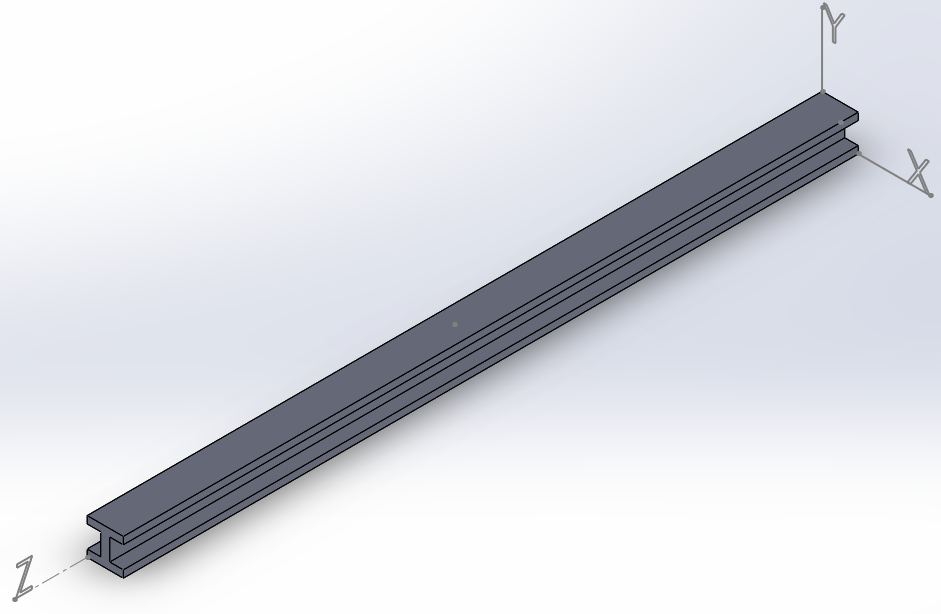
\includegraphics[width=.75\textwidth]{I-BEAM_PLANES}
		\label{fig:I-Beam_Planes}
	\end{figure}
	
	Before experimentation begun, it was theorized that the XZ and YZ beams would behave similarly and that the beams printed with layers in the XY orientation would be the weakest of all of the beams due to the fact that the inter-layer strength is weaker than the strength of the continuous filament layers.
	
	\begin{figure} [H]
		\centering
		\caption{I-Beam Print Orientations}
		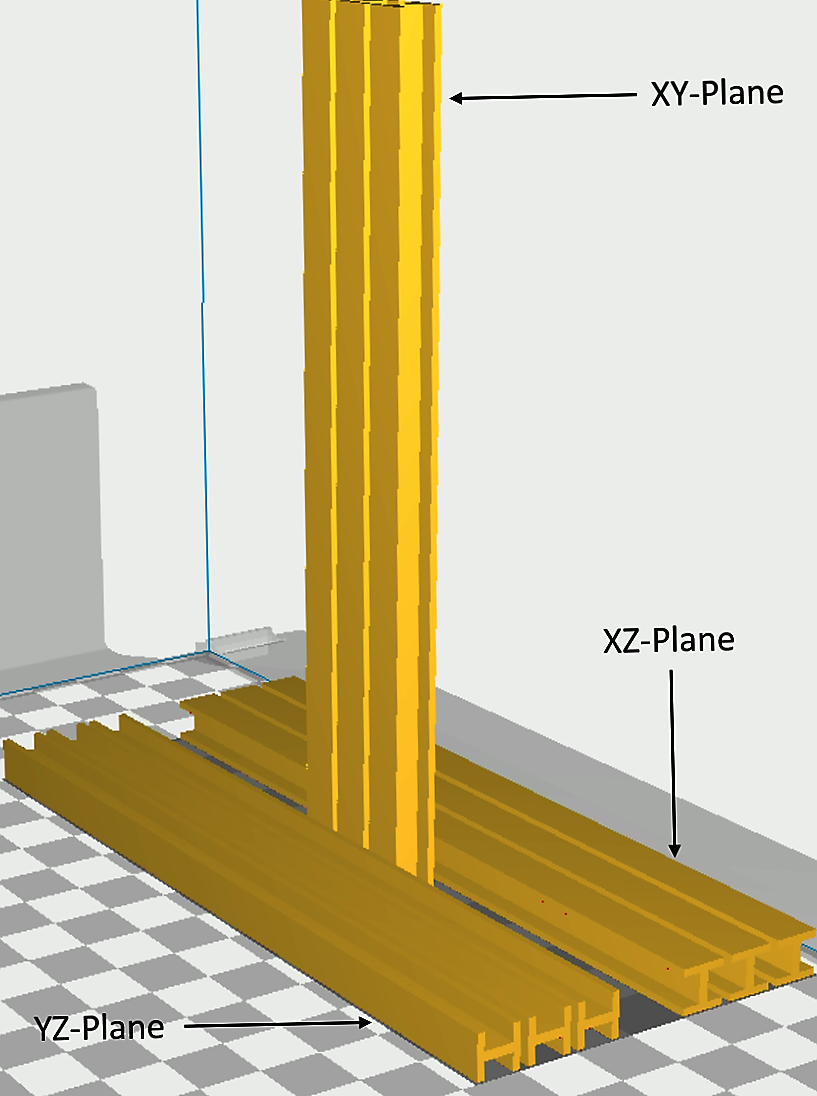
\includegraphics[height=3in]{I-BEAM_CURA}
		\label{fig:I-Beam_Orientations}
	\end{figure}

	Due to the nature of the print orientations, support structure was required to print the XZ and YZ I-Beams which lead to inconsistency in printing close to the nominal beam sizes listed in table \ref{tab:ibeam-nom}. Table \ref{tab:ibeam-dev} notes the average deviation of beams in each print orientation and \ref{tab:ibeam-meas} contains the averaged measurements.
	
	\begin{table} [h]
	\centering
		\begin{tabularx}{\textwidth}{| X | X | X | X | X | X |}
		\hline
			\multicolumn{6}{|c|}{I-Beam Nominal Values} \\ \hline
			\multicolumn{2}{|c|}{BOTTOM FLANGE} & \multicolumn{2}{c|}{TOP FLANGE} & \multicolumn{2}{c|}{WEB}\\ \hline
			 HEIGHT & WIDTH & HEIGHT & WIDTH & HEIGHT & WIDTH \\
			 1.5 & 7.5 & 1.5 & 7.5 & 5 & 1.875 \\ \hline
		\end{tabularx}
		\caption{Nominal I-Beam Measurements}
		\label{tab:ibeam-nom}
	\end{table}
	
	\begin{table} [h]
	\centering
		\begin{tabularx}{\textwidth}{| X | X | X | X | X | X | X |}
		\hline
			\multicolumn{7}{|c|}{I-Beam Measurements} \\ \hline
			& \multicolumn{2}{c|}{BOTTOM FLANGE} & \multicolumn{2}{c|}{TOP FLANGE} & \multicolumn{2}{c|}{WEB}\\ \hline
			Beam & HEIGHT & WIDTH & HEIGHT & WIDTH & HEIGHT & WIDTH \\ \hline
			XY & 1.47 & 7.59 & 1.48 & 7.61 & 4.78 & 1.81 \\ \hline
			XZ & 1.25 & 8 & 1.36 & 7.69 & 4.85 & 1.79 \\ \hline
			YZ & 1.52 & 7.34 & 1.52 & 7.35 & 4.92 & 1.74 \\ \hline
		\end{tabularx}
		\caption{I-Beam Measurements}
		\label{tab:ibeam-meas}
	\end{table}
	
	\begin{table} [h]
	\centering
		\begin{tabularx}{\textwidth}{| X | X | X | X | X | X | X |}
		\hline
			\multicolumn{7}{|c|}{I-Beam Deviation} \\ \hline
			& \multicolumn{2}{c|}{BOTTOM FLANGE} & \multicolumn{2}{c|}{TOP FLANGE} & \multicolumn{2}{c|}{WEB}\\ \hline
			Beam & HEIGHT & WIDTH & HEIGHT & WIDTH & HEIGHT & WIDTH \\ \hline
			XY & 2 & -1.2 & 1.33 & -1.47 & 4.4 & 3.47 \\ \hline
			XZ & 16.67 & -6.67 & 9.33 & -2.53 & 3 & 4.53 \\ \hline
			YZ & -1.33 & 2.13 & -1.33 & 2 & 1.6 & 7.2 \\ \hline
		\end{tabularx}
		\caption{I-Beam Measurement Deviation}
		\label{tab:ibeam-dev}
	\end{table}
	
	When the bending tests were performed on the I-Beam specimens, the top flange of the I beam was facing up regardless of print orientation (the same orientation as the rightmost beams in figure \ref{fig:I-Beam_Orientations}) in order to compare bending for all specimens in the same way. After the data was gathered, the modulus of elasticity of each beam was calculated the same way as in the square and rectangular beams for the linear elastic region captured. For determining the uncertainty, the deformation at 40N was calculated using the average 3.238 GPa modulus of elasticity for 100\% fill PLA and the measured dimensions of the beam and then compared to the actual deformation at $\approx 40N$. 	
	
	The results of the bending tests, listed in table \ref{tab:ibeam_bending_results}, are quite interesting based on previous expectations. The XZ specimens appeared to have the highest modulus of elasticity around 3.134 GPa, which is only $\approx 3.22\%$ lower than the average modulus of 100\% fill PLA beams found in Phase I. The XZ print orientation is the same orientation as the square and rectangular beams, and thus it stands to reason that the I-Beams using the same print orientation have a similar modulus and also shows that print orientation has a significant impact on the strength of the product. The XY samples, which were predicted to be - and are - the weakest have a modulus similar to that of a 50\% infill beam, being only $\approx 2.55\%$ stronger. The YZ beams are in between the strength of the 50\% and 100\% fill beams.

	\begin{table} [h]
		\centering
		\begin{tabularx}{\linewidth}{ | X | X | X | }
		\hline
			Samples & Avg Modulus (GPa) & Uncertainty (\%) \\ \hline
			XY & 2.585 & 26.583 \\
			XZ & 3.134 & 5.199 \\
			YZ & 2.73 & 20.400 \\ \hline
			AVERAGES & 2.816 & 17.394 \\ \hline
		\end{tabularx}
		\caption{I-Beam Bending Test Results}
		\label{tab:ibeam_bending_results}
	\end{table}

It is reasonable to assume that the larger surface area between the layers of the printed beams is the cause of the increased strength due to a larger uniform surface for the next layer to bond to. The following graphs detail the results of individual specimens for the modulus of elasticity and uncertainty in predicting the deformation at 40N.

	\begin{figure} [H]
		\centering
		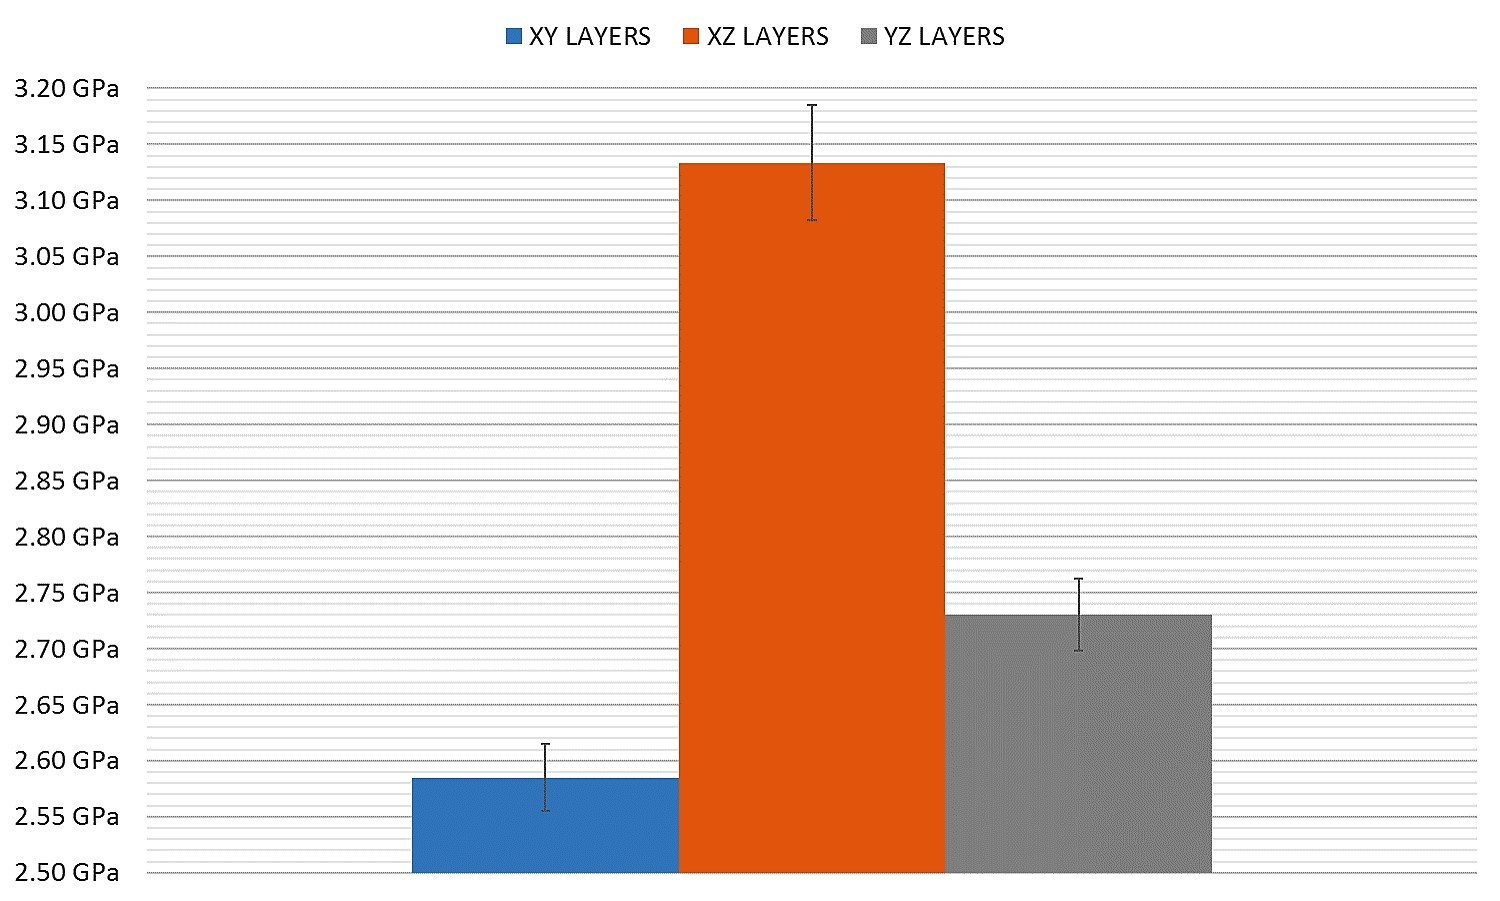
\includegraphics[width=\textwidth]{CHART_I-BEAM_Elasticity}
		\caption{PLA I-Beam Modulus of Elasticity}
		\label{fig:ibeam_Modulus}
	\end{figure}
	
	\begin{figure} [H]
		\centering
		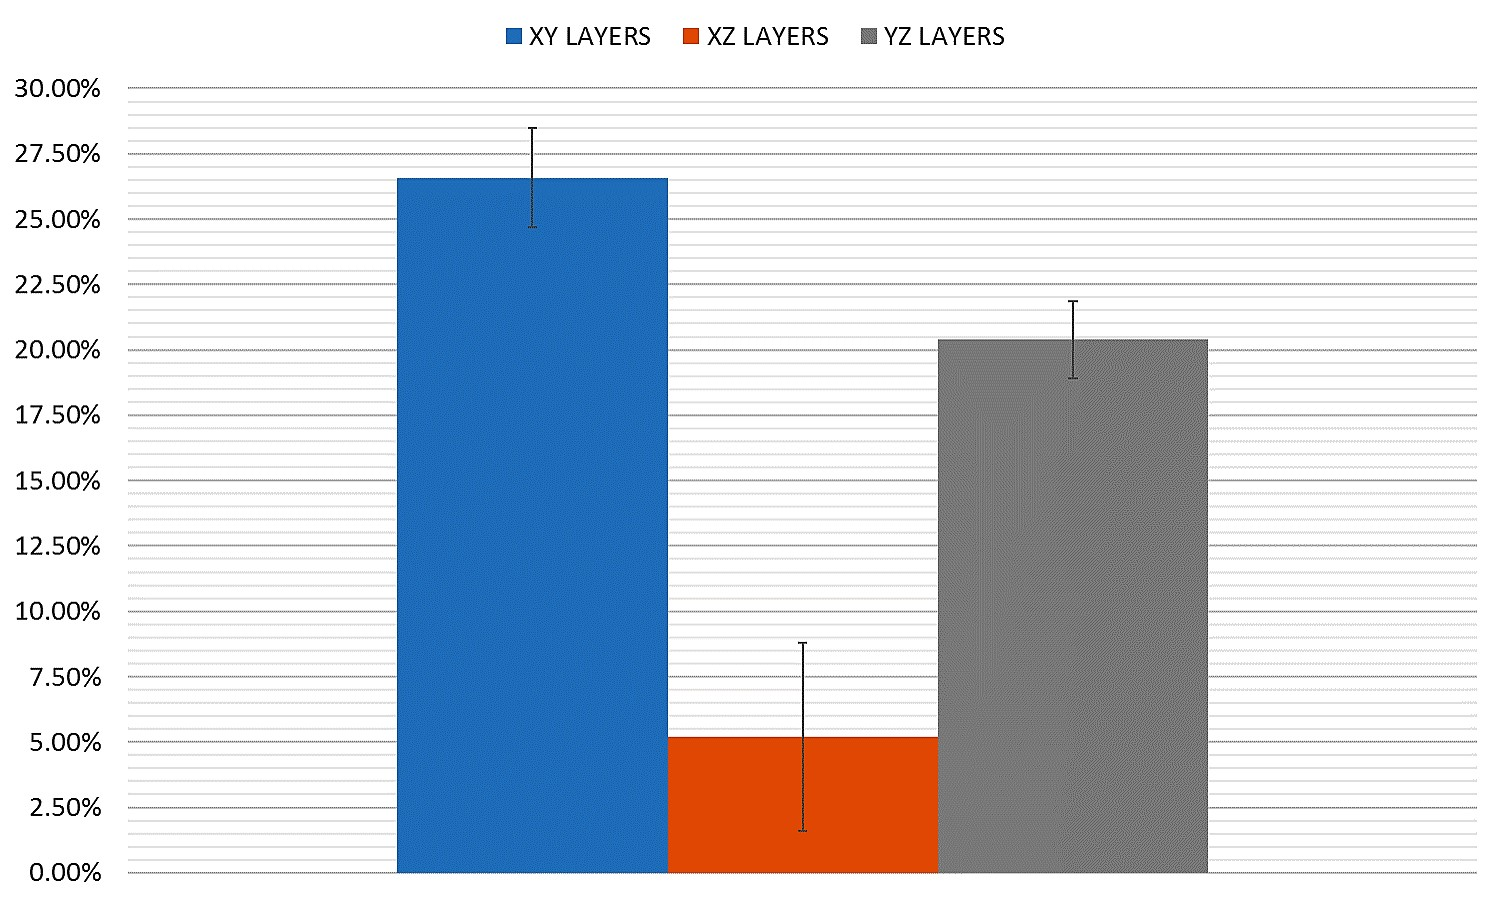
\includegraphics[width=\textwidth]{CHART_I-BEAM_Uncertainty}
		\caption{PLA I-Beam Uncertainty}
		\label{fig:ibeam_Uncertanty}
	\end{figure}

\section{Phase III: Examining UTS Based on Print Orientation}
Phase III was unable to be completed due to scheduling issues with the manufacturing of the grip extensions for the tensile tests. This section is kept here for record keeping and to provide insight into further work.

For our purposes, ASTM D638 was followed with dimensions used for Type I test specimens \citep{ASTMNorma2004} in test specimen design.


\subsection{Design of Grip Extension}
\begin{figure} [H]
\centering
	\caption{\label{ref_label_overall}Grip Extension Clamps}
	\subfloat[Clamp without Bolts]{\label{fig:clamp_no_bolts}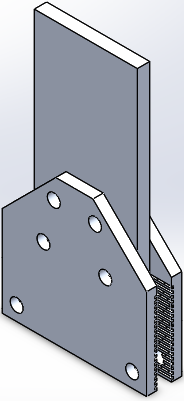
\includegraphics[scale=.7]{Clamp_No_Bolts}}\
	\subfloat[Single Bolt Detail]{\label{fig:clamp_one_bolt}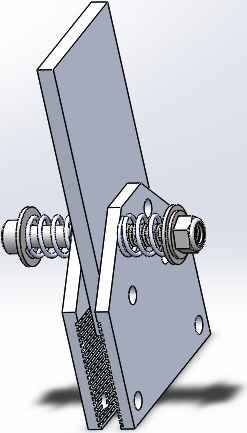
\includegraphics[scale=.65]{Clamp_Single_Bolt}}\
	\subfloat[All Bolts]{\label{fig:clamp_all_bolts}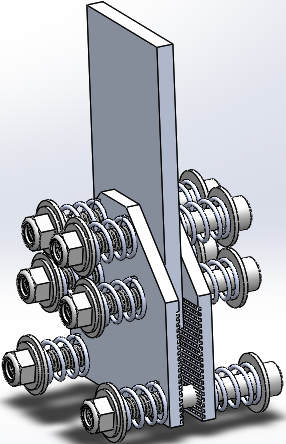
\includegraphics[scale=.65]{Clamp_All_Bolts}}\
\end{figure}

\subsection{Design of Tensile Specimen}

Table \ref{tab:rep_tensile_dimensions} defines the nominal values of the tensile test specimen created in Solidworks. Figure \ref{fig:tens_dim} details the dimensions from \ref{tab:rep_tensile_dimensions} and figure \ref{fig:tens_rend} shows 3D rendering of the specimen taken from Solidworks.

	\begin{table} [H]
		\centering
		\hrule height 2pt 
		\begin{tabularx}{\textwidth}{ | l | X | }
			\multicolumn{2}{|c|}{Type I Tensile Test Specimen Dimensions} \\ \hline
			LO & 200mm\\
			WO & 19mm\\
			L & 57mm\\
			W & 13mm\\
			R & 76mm\\
			T & 3.5mm\\
			G & Unable to provide as no testing was done. \\
		\end{tabularx}
		\hrule height 2pt 
		\caption{Dimensions of Type I Tensile Test Specimens Used}
		\label{tab:rep_tensile_dimensions}
	\end{table}


\begin{figure} [h]
\centering
	\caption{\label{ref_label_overall}Tensile Test Specimens}
	\subfloat[Dimensions Detail]{\label{fig:tens_dim}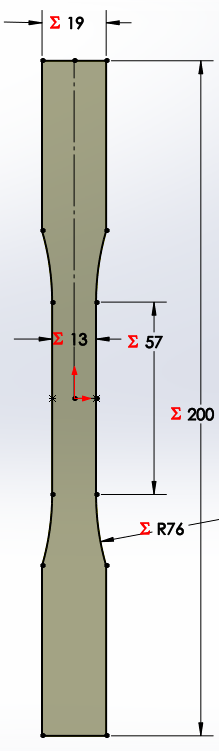
\includegraphics[height=11.5cm]{Tensile_Specimen_Dimensions}}\
	\subfloat[Rendering]{\label{fig:tens_rend}
\includegraphics[height=11.5cm]{Tensile_Specimen_ISO}}\
\end{figure}